% Options for packages loaded elsewhere
% Options for packages loaded elsewhere
\PassOptionsToPackage{unicode}{hyperref}
\PassOptionsToPackage{hyphens}{url}
\PassOptionsToPackage{dvipsnames,svgnames,x11names}{xcolor}
%
\documentclass[
  13.5pt,
  a4paper,
  DIV=11,
  numbers=noendperiod]{scrreprt}
\usepackage{xcolor}
\usepackage{amsmath,amssymb}
\setcounter{secnumdepth}{5}
\usepackage{iftex}
\ifPDFTeX
  \usepackage[T1]{fontenc}
  \usepackage[utf8]{inputenc}
  \usepackage{textcomp} % provide euro and other symbols
\else % if luatex or xetex
  \usepackage{unicode-math} % this also loads fontspec
  \defaultfontfeatures{Scale=MatchLowercase}
  \defaultfontfeatures[\rmfamily]{Ligatures=TeX,Scale=1}
\fi
\usepackage[]{lmodern}
\ifPDFTeX\else
  % xetex/luatex font selection
  \setmainfont[]{Lato}
  \setmonofont[]{Roboto Mono}
\fi
% Use upquote if available, for straight quotes in verbatim environments
\IfFileExists{upquote.sty}{\usepackage{upquote}}{}
\IfFileExists{microtype.sty}{% use microtype if available
  \usepackage[]{microtype}
  \UseMicrotypeSet[protrusion]{basicmath} % disable protrusion for tt fonts
}{}
\makeatletter
\@ifundefined{KOMAClassName}{% if non-KOMA class
  \IfFileExists{parskip.sty}{%
    \usepackage{parskip}
  }{% else
    \setlength{\parindent}{0pt}
    \setlength{\parskip}{6pt plus 2pt minus 1pt}}
}{% if KOMA class
  \KOMAoptions{parskip=half}}
\makeatother
% Make \paragraph and \subparagraph free-standing
\makeatletter
\ifx\paragraph\undefined\else
  \let\oldparagraph\paragraph
  \renewcommand{\paragraph}{
    \@ifstar
      \xxxParagraphStar
      \xxxParagraphNoStar
  }
  \newcommand{\xxxParagraphStar}[1]{\oldparagraph*{#1}\mbox{}}
  \newcommand{\xxxParagraphNoStar}[1]{\oldparagraph{#1}\mbox{}}
\fi
\ifx\subparagraph\undefined\else
  \let\oldsubparagraph\subparagraph
  \renewcommand{\subparagraph}{
    \@ifstar
      \xxxSubParagraphStar
      \xxxSubParagraphNoStar
  }
  \newcommand{\xxxSubParagraphStar}[1]{\oldsubparagraph*{#1}\mbox{}}
  \newcommand{\xxxSubParagraphNoStar}[1]{\oldsubparagraph{#1}\mbox{}}
\fi
\makeatother


\usepackage{longtable,booktabs,array}
\usepackage{calc} % for calculating minipage widths
% Correct order of tables after \paragraph or \subparagraph
\usepackage{etoolbox}
\makeatletter
\patchcmd\longtable{\par}{\if@noskipsec\mbox{}\fi\par}{}{}
\makeatother
% Allow footnotes in longtable head/foot
\IfFileExists{footnotehyper.sty}{\usepackage{footnotehyper}}{\usepackage{footnote}}
\makesavenoteenv{longtable}
\usepackage{graphicx}
\makeatletter
\newsavebox\pandoc@box
\newcommand*\pandocbounded[1]{% scales image to fit in text height/width
  \sbox\pandoc@box{#1}%
  \Gscale@div\@tempa{\textheight}{\dimexpr\ht\pandoc@box+\dp\pandoc@box\relax}%
  \Gscale@div\@tempb{\linewidth}{\wd\pandoc@box}%
  \ifdim\@tempb\p@<\@tempa\p@\let\@tempa\@tempb\fi% select the smaller of both
  \ifdim\@tempa\p@<\p@\scalebox{\@tempa}{\usebox\pandoc@box}%
  \else\usebox{\pandoc@box}%
  \fi%
}
% Set default figure placement to htbp
\def\fps@figure{htbp}
\makeatother





\setlength{\emergencystretch}{3em} % prevent overfull lines

\providecommand{\tightlist}{%
  \setlength{\itemsep}{0pt}\setlength{\parskip}{0pt}}



 


\KOMAoption{captions}{tableheading}
\makeatletter
\@ifpackageloaded{tcolorbox}{}{\usepackage[skins,breakable]{tcolorbox}}
\@ifpackageloaded{fontawesome5}{}{\usepackage{fontawesome5}}
\definecolor{quarto-callout-color}{HTML}{909090}
\definecolor{quarto-callout-note-color}{HTML}{0758E5}
\definecolor{quarto-callout-important-color}{HTML}{CC1914}
\definecolor{quarto-callout-warning-color}{HTML}{EB9113}
\definecolor{quarto-callout-tip-color}{HTML}{00A047}
\definecolor{quarto-callout-caution-color}{HTML}{FC5300}
\definecolor{quarto-callout-color-frame}{HTML}{acacac}
\definecolor{quarto-callout-note-color-frame}{HTML}{4582ec}
\definecolor{quarto-callout-important-color-frame}{HTML}{d9534f}
\definecolor{quarto-callout-warning-color-frame}{HTML}{f0ad4e}
\definecolor{quarto-callout-tip-color-frame}{HTML}{02b875}
\definecolor{quarto-callout-caution-color-frame}{HTML}{fd7e14}
\makeatother
\makeatletter
\@ifpackageloaded{bookmark}{}{\usepackage{bookmark}}
\makeatother
\makeatletter
\@ifpackageloaded{caption}{}{\usepackage{caption}}
\AtBeginDocument{%
\ifdefined\contentsname
  \renewcommand*\contentsname{Table of contents}
\else
  \newcommand\contentsname{Table of contents}
\fi
\ifdefined\listfigurename
  \renewcommand*\listfigurename{List of Figures}
\else
  \newcommand\listfigurename{List of Figures}
\fi
\ifdefined\listtablename
  \renewcommand*\listtablename{List of Tables}
\else
  \newcommand\listtablename{List of Tables}
\fi
\ifdefined\figurename
  \renewcommand*\figurename{Figure}
\else
  \newcommand\figurename{Figure}
\fi
\ifdefined\tablename
  \renewcommand*\tablename{Table}
\else
  \newcommand\tablename{Table}
\fi
}
\@ifpackageloaded{float}{}{\usepackage{float}}
\floatstyle{ruled}
\@ifundefined{c@chapter}{\newfloat{codelisting}{h}{lop}}{\newfloat{codelisting}{h}{lop}[chapter]}
\floatname{codelisting}{Listing}
\newcommand*\listoflistings{\listof{codelisting}{List of Listings}}
\makeatother
\makeatletter
\makeatother
\makeatletter
\@ifpackageloaded{caption}{}{\usepackage{caption}}
\@ifpackageloaded{subcaption}{}{\usepackage{subcaption}}
\makeatother
\usepackage{bookmark}
\IfFileExists{xurl.sty}{\usepackage{xurl}}{} % add URL line breaks if available
\urlstyle{same}
\hypersetup{
  pdftitle={The Complete - Physical Examination Checklists},
  pdfauthor={Ahmad AlHurani},
  colorlinks=true,
  linkcolor={blue},
  filecolor={Maroon},
  citecolor={Blue},
  urlcolor={Blue},
  pdfcreator={LaTeX via pandoc}}


\title{The Complete - Physical Examination Checklists}
\author{Ahmad AlHurani}
\date{2026-01-08}
\begin{document}
\maketitle

\renewcommand*\contentsname{Table of contents}
{
\hypersetup{linkcolor=}
\setcounter{tocdepth}{2}
\tableofcontents
}

\bookmarksetup{startatroot}

\chapter*{Preface to the 2nd version}\label{preface-to-the-2nd-version}
\addcontentsline{toc}{chapter}{Preface to the 2nd version}

\markboth{Preface to the 2nd version}{Preface to the 2nd version}

Welcome to the \emph{\(2nd\) version} of \textbf{The Complete} internal
medicine physical examination checklists!

\section*{What's new}\label{whats-new}
\addcontentsline{toc}{section}{What's new}

\markright{What's new}

\begin{enumerate}
\def\labelenumi{\arabic{enumi}.}
\item
  This eBook is written with \href{https://quarto.org}{Quarto}, for
  smoother experience than ever! No need to use slow notion websites
  anymore!
\item
  Added some important tables and images to help guide you with
  knowledge while performing physical examination
\item
  Refined content, for more cohesive experience!
\item
  Open sourced The Complete!
\end{enumerate}

\bookmarksetup{startatroot}

\chapter{Cardiovascular checklist}\label{cardiovascular-checklist}

\section{WIPPER and the intro}\label{wipper-and-the-intro}

\begin{itemize}
\tightlist
\item[$\square$]
  Introduce yourself and shake hands
\item[$\square$]
  Washing of hands and appropriate hand hygiene
\item[$\square$]
  Asking for permission
\item[$\square$]
  Ensuring the room's privacy
\item[$\square$]
  Ensuring the environmental warmth and good lighting conditions
\item[$\square$]
  Asking for appropriate exposure (\textbf{from the waist and above})
\item[$\square$]
  Asking the patient to be in the appropriate position
  (\textbf{semi-sitting at 45 degrees in bed})
\item[$\square$]
  Relocating to the right side of the patient
\item[$\square$]
  Asking for a chaperon
\item[$\square$]
  ``I have all of my equipment's''
\end{itemize}

\section{General look of the patient}\label{general-look-of-the-patient}

\begin{itemize}
\tightlist
\item[$\square$]
  \textbf{Consciousness, alertness and orientation} of the patient to
  time, place and person (After asking the \href{miscellaneous.qmd}{3
  questions})
\item[$\square$]
  Comment on the patient's \textbf{position and comfort}
\item[$\square$]
  Comment on the patient's \textbf{external devices} status (No oxygen
  masks, nebulizers etc.)
\item[$\square$]
  Comment on \textbf{respiratory rate (Not tachypneic)},
  \textbf{respiratory distress}
\item[$\square$]
  Comment on \textbf{cyanosis}
\item[$\square$]
  Comment on \textbf{edema}
\end{itemize}

\section{Vital Signs}\label{vital-signs}

\begin{itemize}
\tightlist
\item[$\square$]
  Make sure you know the \href{miscellaneous.qmd}{6 vital signs}
\end{itemize}

\section{Hands - Inspection}\label{hands---inspection}

Starting with the hand

\begin{itemize}
\tightlist
\item[$\square$]
  No \textbf{cyanosis}
\item[$\square$]
  No \textbf{pallor}
\item[$\square$]
  No \textbf{palmar erythema}
\item[$\square$]
  No \textbf{petechial rash}
\item[$\square$]
  No \textbf{Xanthomata} (Hyper-lipidemia)
\item[$\square$]
  No \textbf{Janeway lesions} (painless, thenar region) (Infective
  endocarditis)
\item[$\square$]
  No \textbf{Osler's nodes} (painful, tip of fingers) (Infective
  endocarditis)
\item[$\square$]
  No \textbf{tar staining}
\item[$\square$]
  No \textbf{IV drug abuse signs}
\end{itemize}

Moving on to the nails

\begin{itemize}
\tightlist
\item[$\square$]
  No \textbf{finger clubbing}
\item[$\square$]
  No \textbf{splinter hemorrhages} (Infective endocarditis)
\end{itemize}

End this section by examining for tremor

\begin{itemize}
\tightlist
\item[$\square$]
  Examine for \textbf{fine tremor}
\end{itemize}

\section{Hands - Palpation}\label{hands---palpation}

\begin{itemize}
\tightlist
\item[$\square$]
  Check hands' \textbf{temperature, dry/sweatiness}
\item[$\square$]
  Check \textbf{Capillary refill} (\textless2 seconds is a normal
  capillary refill time)
\end{itemize}

Check pulses bilaterally, details below\\
All pulses are done with 2 fingers, \textbf{except for radial;}

\section{Radial pulse}\label{radial-pulse}

\begin{itemize}
\tightlist
\item[$\square$]
  Radial pulse; \textbf{using 3 fingers}, \textbf{lateral to flexor
  carpi radialis}, after 1 minute (do 15sec), comment on the rate,
  rhythm, volume, character and compressibility.
\item[$\square$]
  Check both radial pulses simultaneously to assess
  ``\textbf{Radio-radial delay}'', a sign for aortic dissection
\item[$\square$]
  Check radial and femoral pulses simultaneously to assess
  ``\textbf{Radio-femoral delay}'', a sign for aortic coarctation (ONLY
  MENTION)
\item[$\square$]
  Calculate \textbf{pulse deficit}, we don't do this during exams
  (mention it), but a difference of \textbf{+10 BPM} is abnormal
  (Associated with atrial fibrillation)
\item[$\square$]
  Now ask the patient about shoulder pain first, if none is present,
  \textbf{elevate hand above level of patient's head while checking the
  radial pulse}, to check for ``\textbf{Collapsing pulse}'' (Aortic
  regurgitation)
\item[$\square$]
  Don't forget to comment your findings, mention the HR measured,
  regular rhythm, normal volume, normal character, compressible, no
  radio-radial/radio-femoral delays, no pulse deficit, no collapsing
  pulse.
\end{itemize}

\section{Brachial pulse}\label{brachial-pulse}

\begin{itemize}
\tightlist
\item[$\square$]
  Using \textbf{2 fingers}, assess the brachial pulse \textbf{medial to
  the biceps tendon} in antecubital fossa. (Bilaterally)
\item[$\square$]
  Mention rate, rhythm, volume, character and compressibility
\end{itemize}

\section{Carotid pulse}\label{carotid-pulse}

\begin{itemize}
\tightlist
\item[$\square$]
  Using \textbf{2 fingers}, gently assess the carotid pulse
  \textbf{anterior to sternocleidomastoid near the jaw}.
\item[$\square$]
  Bilaterally,
  \texttt{but\ never\ feel\ both\ sides\ at\ the\ same\ time} as that
  might trigger vasovagal attack, comment on rate, rhythm, volume,
  character and compressibility
\item[$\square$]
  Ask the patient to \textbf{hold his breath}, and auscultate for the
  bruit
\item[$\square$]
  Comment on the bruit
\end{itemize}

\subsubsection{Femoral (mention only), posterior tibial and dorsalis
pedis are done in PVS. We do them if the station was a focused pulses
station}\label{femoral-mention-only-posterior-tibial-and-dorsalis-pedis-are-done-in-pvs.-we-do-them-if-the-station-was-a-focused-pulses-station}

\section{Face}\label{face}

\begin{itemize}
\tightlist
\item[$\square$]
  Check eyelids for \textbf{xanthelasmata} (Hyper-lipidemia)
\item[$\square$]
  Check iris for \textbf{corneal arcus} (Hyper-lipidema)
\item[$\square$]
  Check conjunctiva for \textbf{pallor and petechial hemorrhage}
  (Infective endocarditis)
\item[$\square$]
  Mention that you need \textbf{fundoscopy} to check for \textbf{roth
  spots} (Infective endocarditis), or \textbf{HTN/DM changes}
\item[$\square$]
  Check for \textbf{malar flush} on cheeks (Mitral valve stenosis)
\item[$\square$]
  Check for any signs of \textbf{central cyanosis} (Under the tongue),
  \textbf{peripheral cyanosis} (On the lips)
\end{itemize}

\section{JVP Examination}\label{jvp-examination}

As JVP is very important and might be a full station on its own, make
sure you're ready for it.

\subsection{Inspection}\label{inspection}

\begin{itemize}
\tightlist
\item[$\square$]
  Rest the patient's head on a pillow (Make sure its rested, we need a
  relaxed sternocleidomastoid), ask him to \textbf{turn his head
  slightly to the left}, using a torch, try to find JVP pulsation.
\item[$\square$]
  Comment, \textbf{double peaked, inward pulsating JVP}
\end{itemize}

\subsection{Palpation}\label{palpation}

\begin{itemize}
\tightlist
\item[$\square$]
  After doing the \href{miscellaneous.qmd}{usuals for any palpation},
  try to palpate it
\end{itemize}

JVP is \textbf{normally impalpable}, so make this comment and move on

\begin{itemize}
\tightlist
\item[$\square$]
  \textbf{Compress the root of the neck, JVP should disappear}, comment
  that it disappeared after compressing root of the neck
\item[$\square$]
  Ask the patient to \textbf{lie flat → Increased JVP} (comment)
\item[$\square$]
  Ask the patient to \textbf{sit straight → Decreased JVP} (comment)
\item[$\square$]
  Ask the patient to take a \textbf{deep inspiration → Decreased JVP}
  (comment)
\item[$\square$]
  Check \textbf{abdominojugular reflux}, press (\textbf{while gradually
  increasing pressure}) on the Rt upper quadrant for 30 seconds (don't
  do full 30 of course), on a positive test (normally positive),
  \textbf{JVP increases} (comment whether positive or negative reflux)
\end{itemize}

\subsection{Measuring JVP}\label{measuring-jvp}

\begin{itemize}
\tightlist
\item[$\square$]
  Use a ruler, put it on the sternal angle (Straight with the ground not
  patient's body), assess using a straight object that's put on the
  highest pulsation you see of the JVP, measure on the ruler and add 5cm
  and comment on the measured JVP (\textbf{Normally it's
  \textless9cmH20})
\end{itemize}

\section{Precordium Examination}\label{precordium-examination}

\subsection{Inspection}\label{inspection-1}

From the foot of the bed;

\begin{itemize}
\tightlist
\item[$\square$]
  First ask the patient to take a deep breath
\item[$\square$]
  Comment ``\textbf{Symmetrical chest with no visible deformities,
  bilateral movement of chest with respiration}''
\end{itemize}

From the right side of the pt;

\begin{itemize}
\tightlist
\item[$\square$]
  Check for \textbf{scars}, make sure you know what scars mean;

  \begin{enumerate}
  \def\labelenumi{\arabic{enumi}.}
  \tightlist
  \item
    \textbf{Midsternotomy} is for \textbf{CABG}\\
  \item
    \textbf{Left submammary} is for \textbf{mitral valvotomy}\\
  \item
    \textbf{Infraclavicular} is for \textbf{pacemakers}\\
    And mention \textbf{no scars}
  \end{enumerate}
\item[$\square$]
  Mention \textbf{no swellings, visible masses, dilated veins.}
\item[$\square$]
  Mention \textbf{normal hair distribution}
\item[$\square$]
  Using the \textbf{torch}, mention afterwards that you see \textbf{no
  visible pulsation/no visible apex beat}
\end{itemize}

\subsection{Palpation}\label{palpation-1}

\begin{itemize}
\tightlist
\item[$\square$]
  Do the \href{miscellaneous.qmd}{usuals for palpation}
\item[$\square$]
  Generally palpate the chest, don't miss any point, use your whole hand
\item[$\square$]
  Comment \textbf{no palpable masses, no tenderness}
\end{itemize}

\textbf{Apex beat}

\begin{itemize}
\tightlist
\item[$\square$]
  Try to find it using your \textbf{whole hand}
\item[$\square$]
  Try to find it using \textbf{2 fingers} (roll the patient to the left
  side if you couldn't find it)
\item[$\square$]
  Locate it → which intercostal space, is it midclavicular?
\item[$\square$]
  Comment; \textbf{gently tapping apex beat, located in the 5th
  intercostal space, midclavicular line.}
\end{itemize}

\textbf{Heaves}

\begin{itemize}
\tightlist
\item[$\square$]
  Using your \textbf{hand's heel}, ask the patient to expire and hold
  his breath, assess both \textbf{right ventricular heave (lower left
  sternal angle)}, and \textbf{left ventricular heave (apex, hence
  ``apical heave'')}
\item[$\square$]
  Comment! \textbf{No right or left ventricular heaves}
\end{itemize}

\textbf{Thrills}

\begin{itemize}
\tightlist
\item[$\square$]
  Using your \textbf{flat fingers}; not the tips nor the base, check for
  thrills in 4 locations; apex, parasternal, right and left second
  intercostals.
\item[$\square$]
  Comment! \textbf{No thrills}
\end{itemize}

\subsection{Auscultation}\label{auscultation}

\begin{figure}[H]

{\centering \pandocbounded{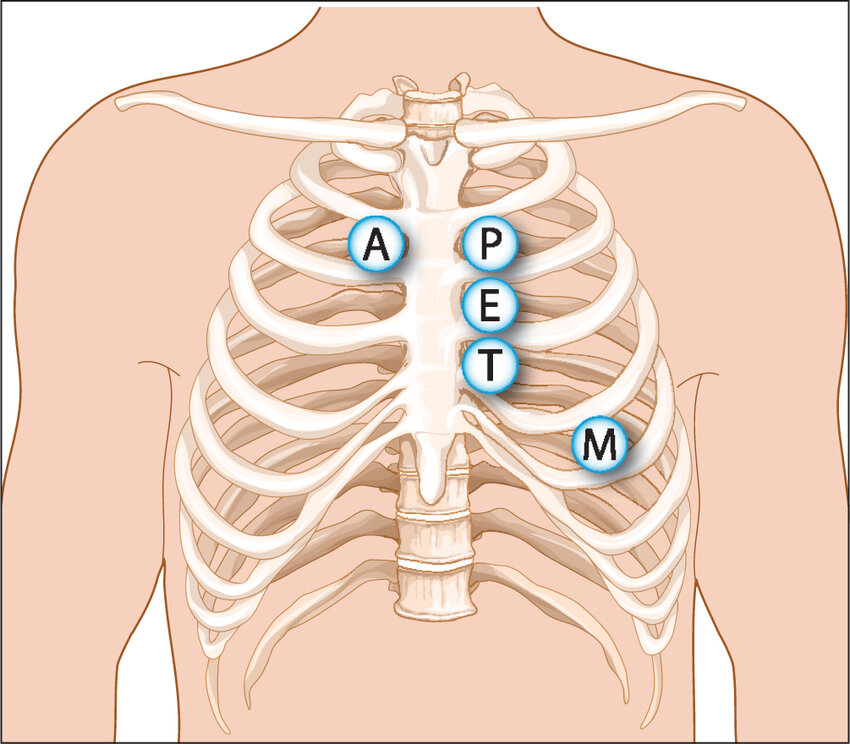
\includegraphics[keepaspectratio]{cvs10.png}}

}

\caption{Auscultation spots}

\end{figure}%

Differentiate S1/S2 by \textbf{feeling carotid pulse while auscultating
the patient}

\begin{itemize}
\tightlist
\item
  First, with the diaphragm, 4 valvular spots and 2 radiation spots

  \begin{itemize}
  \tightlist
  \item[$\square$]
    4 Valvular spots, \textbf{mitral, tricuspid, aortic and pulmonary}
  \item[$\square$]
    1 Carotid, for \textbf{radiation of aortic stenosis}
  \item[$\square$]
    1 Left axilla, for \textbf{radiation of mitral regurgitation}
  \end{itemize}
\item
  Second, with the bell, 4 spots

  \begin{itemize}
  \tightlist
  \item[$\square$]
    4 Valvular spots (some only use the bell for mitral and tricuspid,
    you'll not be penalized for more spots anyway)
  \end{itemize}
\item
  Last, finish with 2 maneuvers

  \begin{itemize}
  \tightlist
  \item[$\square$]
    \textbf{Aortic regurgitation}, using the diaphragm, ask the patient
    to sit straight and then lean forward, examine (aortic area), and
    \textbf{Erb's area}.
  \item[$\square$]
    \textbf{Mitral stenosis}, using the bell, ask the patient to roll to
    his left side and then put the bell on the apex.
  \item[$\square$]
    Comment on the whole auscultation; ``\textbf{Normal S1,S2, no S3,S4,
    normal physiological splitting of S2, no murmurs, no added sounds
    like opening snap, ejection click or friction rub}''
  \end{itemize}
\end{itemize}

\section{Ending the station}\label{ending-the-station}

\pandocbounded{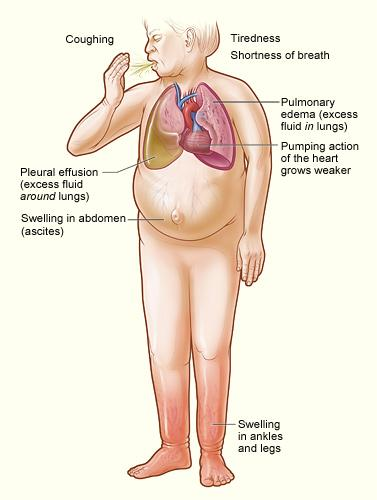
\includegraphics[keepaspectratio]{cvs12.png}}

\begin{itemize}
\tightlist
\item[$\square$]
  I will auscultate \textbf{lung bases for crackles} (Heart failure -
  Pulmonary edema)
\item[$\square$]
  I will examine the \textbf{abdomen for ascites; hepatomegaly, sacral
  edema}
\item[$\square$]
  I will examine \textbf{lower limb for edema, ulcers, pulses}
\end{itemize}

\bookmarksetup{startatroot}

\chapter{Respiratory checklist}\label{respiratory-checklist}

\section{WIPPER and the intro}\label{wipper-and-the-intro-1}

\begin{itemize}
\tightlist
\item[$\square$]
  Introduce yourself and shake hands
\item[$\square$]
  Washing of hands and appropriate hand hygiene
\item[$\square$]
  Asking for permission
\item[$\square$]
  Ensuring the room's privacy
\item[$\square$]
  Ensuring the environmental warmth and good lighting conditions
\item[$\square$]
  Asking for appropriate exposure (\textbf{from the waist and above})
\item[$\square$]
  Asking the patient to be in the appropriate position
  (\textbf{simi-sitting at 45 degrees in bed})
\item[$\square$]
  Relocating to the right side of the patient
\item[$\square$]
  Asking for a chaperon
\item[$\square$]
  ``I have all of my equipment's''
\end{itemize}

\section{General look of the
patient}\label{general-look-of-the-patient-1}

\begin{itemize}
\tightlist
\item[$\square$]
  \textbf{Consciousness, alertness and orientation} of the patient to
  place, time and person (Asking the 3 questions) - \textbf{in RS,}
  \emph{disorientation is a sign for CO2 retention, it causes confusion
  (Hypercapnia)}
\item[$\square$]
  Commenting on the \textbf{patient's position and comfort}
\item[$\square$]
  Commenting on the patient's \textbf{external devices} status (No
  oxygen masks, nebulizers etc.)
\item[$\square$]
  Commenting on \textbf{respiratory rate (Not tachypneic)},
  \textbf{respiratory distress} (Mention these 2 signs)

  \begin{enumerate}
  \def\labelenumi{\arabic{enumi})}
  \tightlist
  \item
    No apparent use of \textbf{accessory muscles} for breathing like
    \emph{sternocleidomastoid, trapezius and scalene)}\\
  \item
    No Indrawing of \textbf{intercostal spaces}
  \end{enumerate}
\item[$\square$]
  Commenting on \textbf{cyanosis}
\item[$\square$]
  No abnormal \textbf{sounds}
\item[$\square$]
  No abnormal \textbf{odors}
\end{itemize}

\section{Vital signs}\label{vital-signs-1}

\begin{itemize}
\item[$\square$]
  Make sure you know the 6 vital signs
\item[$\square$]
  What is \textbf{pulsus paradoxus}?
\item
  \textbf{Pulsus paradoxus} is a more marked inspiratory decrease in
  arterial pressure exceeding 10 mmHg
\item
  \textbf{BMI is vital} in respiratory system, obese patients may get
  \emph{obstructive sleep apnea}
\item
  \textbf{Weight loss} in COPD patients \textbf{increases risk of
  morbidities} (++inflammatory cytokines = ++metabolic rate)
\end{itemize}

\section{Hands examination}\label{hands-examination}

Starting with the still hand

\begin{itemize}
\tightlist
\item[$\square$]
  No \textbf{deformities} / \textbf{amputations}
\item[$\square$]
  No \textbf{palmar erythema}
\item[$\square$]
  No \textbf{pallor}
\item[$\square$]
  No \textbf{scars, swellings and no visible masses}
\item[$\square$]
  No \textbf{tar staining}
\item[$\square$]
  No \textbf{muscle wasting} (thenar and hypothenar)
\end{itemize}

Moving on to the nails

\begin{itemize}
\tightlist
\item[$\square$]
  No \textbf{clubbing} (May be asked to do the 3 tests, \textbf{nail bed
  angle} / \textbf{schamroth's window} / \textbf{fluctuations})
\item[$\square$]
  No nail deformities like \textbf{yellow nail syndrome}
\end{itemize}

Hand palpation and radial pulse

\begin{itemize}
\tightlist
\item[$\square$]
  After doing the \href{miscellaneous.qmd}{usual for palpation}; check
  \textbf{temperature + dryness/sweatiness}
\item[$\square$]
  Test for \textbf{HPOA} (\textbf{Hypertrophic pulmonary
  osteoarthropathy}) (\textbf{Wrist tenderness})
\item[$\square$]
  Test for \textbf{Capillary refill} (1 minute pressure on the nail,
  refill in \textless2 seconds)
\item[$\square$]
  Check \textbf{radial pulse}
\end{itemize}

End this section by examining for tremor

\begin{itemize}
\tightlist
\item[$\square$]
  Test for \textbf{fine tremor}
\item[$\square$]
  Test for \textbf{asterixis (Flapping tremor)} \textasciitilde{}
  \emph{(CO2 retention)}
\end{itemize}

\section{Face examination}\label{face-examination}

\begin{itemize}
\tightlist
\item[$\square$]
  Comment on having no \textbf{plethoric face}
\item[$\square$]
  Comment on having no \textbf{face swelling}
\end{itemize}

By examining the \textbf{eye}, make these 3 comments:

\begin{itemize}
\tightlist
\item[$\square$]
  No \textbf{jaundice} (Examining the sclera)
\item[$\square$]
  No \textbf{pallor} (Examining the color of conjunctiva)
\item[$\square$]
  No \textbf{conjunctival edema}
\item[$\square$]
  Check for \textbf{Horner syndrome} (3 signs; \textbf{ptosis},
  \textbf{meiosis}, \textbf{anhidrosis})
\item[$\square$]
  No \textbf{nasal flaring}
\item[$\square$]
  No \textbf{pursed lips}
\item[$\square$]
  Comment on \textbf{cyanosis} (Peripheral on lips, central under the
  tongue)
\item[$\square$]
  Comment on \textbf{good oral and dental hygiene}
\end{itemize}

\section{Neck examination}\label{neck-examination}

\begin{itemize}
\tightlist
\item[$\square$]
  No \textbf{scars, swellings, visible masses}
\item[$\square$]
  No visible \textbf{dilated veins}
\item[$\square$]
  Mention examining the \textbf{JVP} (SKIP)
\item[$\square$]
  Mention examining the \textbf{cervical lymph nodes} (SKIP)
\end{itemize}

\section{Chest Inspection}\label{chest-inspection}

\textbf{First, relocate to the foot of the bed}

\begin{itemize}
\tightlist
\item[$\square$]
  Comment on symmetrical elliptical chest in cross section
  \textbf{(Shape)}
\item[$\square$]
  Before chest expansion,
  \texttt{ask\ the\ patient\ to\ **take\ a\ deep\ breath\ first**!}
\item[$\square$]
  Comment on \textbf{bilaterally symmetrical} \textbf{chest expansion}
\item[$\square$]
  No \textbf{chest deformities} (kyphosis, scoliosis, pectus carinatum,
  pectus excavatum, barrel chest)
\item[$\square$]
  Normal bilaterally symmetrical \textbf{breathing pattern} that's
  \textbf{Abdomeno-Thoracic}
\item[$\square$]
  \textbf{Pemberton sign} (raise both of your hands, wait for facial
  plethora) to check for SVC obstruction
\end{itemize}

\textbf{From the right side of the patient}

\begin{itemize}
\tightlist
\item[$\square$]
  No \textbf{Scars, swellings, visible masses}
\item[$\square$]
  No skin \textbf{lesions} \textasciitilde{} \textbf{Subcutaneous
  nodules} (Malignancy)
\item[$\square$]
  No \textbf{visible dilated veins}
\item[$\square$]
  Normal \textbf{hair distribution}
\item[$\square$]
  Check the \textbf{axilla} too!!!!
\end{itemize}

\section{Chest Palpation}\label{chest-palpation}

Do the \href{miscellaneous.qmd}{usuals for any palpation} and then;

\begin{enumerate}
\def\labelenumi{\arabic{enumi})}
\tightlist
\item
  \textbf{General palpation:}
\end{enumerate}

\begin{itemize}
\tightlist
\item[$\square$]
  Palpate using the palm of the hand around the chest
\end{itemize}

Mention that you found:

\begin{itemize}
\tightlist
\item[$\square$]
  No \textbf{tenderness}
\item[$\square$]
  No \textbf{subcutaneous emphysema}
\item[$\square$]
  No \textbf{palpable masses}
\end{itemize}

\begin{enumerate}
\def\labelenumi{\arabic{enumi})}
\setcounter{enumi}{1}
\tightlist
\item
  \textbf{Upper mediastinum palpation:}
\end{enumerate}

\begin{itemize}
\tightlist
\item[$\square$]
  Using 3 fingers, check for \textbf{tracheal deviation} (comment that
  it's centralized)
\item[$\square$]
  Ask the patient to take a deep inspiration, to check for
  \textbf{tracheal tug}
\item[$\square$]
  Comment on no tracheal tug
\item[$\square$]
  Measure the \textbf{crico-sternal distance} (Normally; 3 to 4 fingers)
\end{itemize}

\begin{enumerate}
\def\labelenumi{\arabic{enumi})}
\setcounter{enumi}{2}
\tightlist
\item
  \textbf{Lower mediastinum palpation:}
\end{enumerate}

\begin{itemize}
\tightlist
\item[$\square$]
  Using \textbf{palm of the hand} at first, then \textbf{two fingers};
  \textbf{locate the Apex beat}
\item[$\square$]
  \textbf{After locating it}, start from the sternal angle, horizontal
  with 2nd intercostal space, count and mention the position of apex
  beat (Normal pos is in 5th intercostal space, mid clavicular line)
\item[$\square$]
  Mention that it's \textbf{gently-tapping apex beat!} / gently raises
  the pulsating finger!
\item[$\square$]
  Using heel of the hand; putting it in the \textbf{lower-left sternal
  angle}; locate the \textbf{right ventricular heave}, should be
  negative (sign of \emph{severe pulmonary hypertension})
\end{itemize}

\begin{enumerate}
\def\labelenumi{\arabic{enumi})}
\setcounter{enumi}{3}
\tightlist
\item
  \textbf{Last tests}
\end{enumerate}

\begin{itemize}
\tightlist
\item[$\square$]
  Test for \textbf{tactile vocal fremitus} by using palm of the hand on
  4 points anteriorly, 4 points posteriorly, 3 points laterally. (SAY
  اربعة واربعين)
\item[$\square$]
  Comment on \textbf{normal bilaterally symmetrical tactile vocal
  fremitus}
\item[$\square$]
  Test for chest expansion, \textbf{upper and lower anteriorly}
\item[$\square$]
  Test for chest expansion, \textbf{only once posteriorly}
\end{itemize}

Normal chest expansion is around 2.5cm on each side!

\begin{itemize}
\tightlist
\item[$\square$]
  Comment on normal bilaterally symmetrical \textbf{chest expansion}
\end{itemize}

\section{Chest Percussion}\label{chest-percussion}

\textbf{Percuss bilaterally for each spot;}

\begin{itemize}
\tightlist
\item[$\square$]
  Start percussing for the \textbf{lung apex} (left hand pointing
  posteriomedial)
\item[$\square$]
  Percuss on the \textbf{clavicle heads} with \textbf{only your right
  middle finger}
\item[$\square$]
  Percuss from the 2nd intercostal space and keep going space by space
\item[$\square$]
  Anteriorly and on the right, \textbf{find the liver's level}
\item[$\square$]
  \textbf{Percuss both lateral sides of the chest}
\item[$\square$]
  \textbf{Percuss posteriorly}
  (`\texttt{Ask\ patient\ to\ hug\ a\ magical\ pillow!})
\item[$\square$]
  \textbf{Calculate diaphragmatic excursion on each side}! (Remember
  what we ask the patient for \textasciitilde{} deep inspiration etc) -
  normal distance 5-8cm
\end{itemize}

\textbf{Comment on having normal, bilaterally symmetrical resonant
percussion note}

\section{Chest Auscultation}\label{chest-auscultation}

\textbf{Get your stethoscope ready!} set it to use the diaphragm (large
one), test that by \textbf{GENTLY tapping it}, \textbf{WARM it} by
rubbing it with your hand

\begin{itemize}
\tightlist
\item[$\square$]
  Ask the patient to \textbf{face the other side} (his left side; you're
  on the right side right? wait right?!)
\item[$\square$]
  Ask the patient to take a \textbf{deep inspiration and expiration}
  every time the stethoscope touches him (from the mouth and not the
  nose)
\item[$\square$]
  Listen to chest sounds using \textbf{diaphragm} of stethoscope on the
  lung apex, anterior chest, lateral and posterior chest (again,
  bilaterally on each spot)
\item[$\square$]
  Comment on normal \textbf{bilaterally symmetrical vesicular breathing
  sound with inspiration phase longer than expiration}
\item[$\square$]
  Comment on \textbf{good bilateral} \textbf{air entry}
\item[$\square$]
  Comment on having \textbf{no added sounds} (examples; \textbf{wheeze,
  crackles, pleural rub})
\end{itemize}

\textbf{Vocal resonance (Non-tactile)}

\begin{itemize}
\tightlist
\item[$\square$]
  Listen to the chest again, same positions but instead of deep insp/exp
  ask the patient to say اربعة واربعين
\item[$\square$]
  Comment on \textbf{normal bilateral vocal resonance}
\end{itemize}

\textbf{Whispered pectoriloquy}

\begin{itemize}
\tightlist
\item[$\square$]
  Listen to the chest again, same positions but instead of deep insp/exp
  ask the patient to WHISPER (يهمس اربعة واربعين)
\item[$\square$]
  Comment on hearing \textbf{no whispering pectoriloquy}
\end{itemize}

\textbf{Aeogophony}

\begin{itemize}
\tightlist
\item[$\square$]
  Listen to the chest again, same positions but instead of deep insp/exp
  ask the patient to say E
\item[$\square$]
  Comment on hearing \textbf{no aeogophony}
\end{itemize}

\section{\texorpdfstring{\textbf{ENDING the
station!}}{ENDING the station!}}\label{ending-the-station-1}

\begin{itemize}
\tightlist
\item[$\square$]
  I would like to request \textbf{ENT examination} for my patient to
  check his upper airways
\item[$\square$]
  I would like to examine the abdomen for \textbf{hepato-spleenomegaly}
  and \textbf{ascitis}
\item[$\square$]
  I would like to examine lower limbs for \textbf{edema},
  \textbf{erythema nodosum}, signs of \textbf{DVT}
\end{itemize}

\bookmarksetup{startatroot}

\chapter{Gastrointestinal checklist}\label{gastrointestinal-checklist}

\section{WIPPER and the intro}\label{wipper-and-the-intro-2}

\begin{itemize}
\tightlist
\item[$\square$]
  Introduce yourself and shake hands
\item[$\square$]
  Washing of hands and appropriate hand hygiene
\item[$\square$]
  Asking for permission
\item[$\square$]
  Ensuring the room's privacy
\item[$\square$]
  Ensuring the environmental warmth and good lighting conditions
\item[$\square$]
  Asking for appropriate exposure (from the \textbf{xiphisternum} to the
  \textbf{symphysis pubis}) (nipples to mid thigh originally)
\item[$\square$]
  Asking the patient to be in the appropriate position (flat with \(1\)
  or \(2\) pillows \textasciitilde{} around \(10-15\) degrees)
\item[$\square$]
  Relocating to the right side of the patient
\item[$\square$]
  Asking for a chaperon
\item[$\square$]
  ``I have all of my equipment's''
\end{itemize}

\section{General look of the
patient}\label{general-look-of-the-patient-2}

\begin{itemize}
\tightlist
\item[$\square$]
  \textbf{Consciousness, alertness and orientation} of the patient to
  time, place and person (After asking
  \href{miscellaneous.qmd}{\emph{the} \(3\) questions)}
\item[$\square$]
  Comment on the patient's \textbf{position} and \textbf{comfort}
\item[$\square$]
  Comment on the patient's \textbf{external devices} status, such as
  \textasciitilde{} stomas, drains, catheters, etc
\item[$\square$]
  Patient is not in \textbf{respiratory distress}, not
  \textbf{tachycardic}, if he's \textbf{cachectic} or \textbf{obese}
\item[$\square$]
  No \textbf{skin redundancy}
\end{itemize}

\section{Vital signs}\label{vital-signs-2}

\begin{itemize}
\tightlist
\item[$\square$]
  Make sure you know the \href{miscellaneous.qmd}{\(6\) vital signs}
\item[$\square$]
  Take height and weight to calculate BMI and assess nutritional status
  of the pt
\end{itemize}

\section{Hands}\label{hands}

Starting with a quick glance at the nails:

\begin{itemize}
\tightlist
\item[$\square$]
  No \textbf{finger clubbing}
\item[$\square$]
  No \textbf{koilonychia} (\emph{IDA}), \textbf{leukonychia}
  (\emph{Hypoalbuminemia})
\end{itemize}

Moving to the still-hand-examination:

\begin{itemize}
\tightlist
\item[$\square$]
  No \textbf{dupuytren's contracture} (\emph{Alcohol related chronic
  liver diseases})
\item[$\square$]
  No \textbf{muscle wasting}
\item[$\square$]
  No \textbf{tar stain}
\item[$\square$]
  No \textbf{palmar erythema}
\item[$\square$]
  No \textbf{pallor}
\item[$\square$]
  No \textbf{I.V drug abusing marks}
\end{itemize}

Moving to the palpation part of hand examination + tests:

\begin{itemize}
\tightlist
\item[$\square$]
  Do the \textbf{\href{miscellaneous.qmd}{usuals for palpation}}, then
  palpate hand's \textbf{temperature} and comment on
  \textbf{dryness/sweatiness} (Bilaterally)
\item[$\square$]
  Test for \textbf{flapping tremor} (\emph{Asterixis})
  \texttt{(Don’t\ apply\ resistance!!)}
\end{itemize}

\section{Face}\label{face-1}

Eyes;

\begin{itemize}
\tightlist
\item[$\square$]
  Ask the patient to look down and retract upper eyelid to expose sclera
  \emph{\{scleral icterus\}}, No \textbf{jaundice}
\item[$\square$]
  Do the opposite of the previous tick, examine conjunctiva for
  \textbf{pallor}
\end{itemize}

Cheeks and lips;

\begin{itemize}
\tightlist
\item[$\square$]
  No visible \textbf{sialadenitis or sialadenosis (Parotid swellings;
  \emph{chronic alcohol abuse}, \emph{bulimia nervosa})}
\item[$\square$]
  No \textbf{spider nevi} \texttt{(Better\ mentioned\ on\ chest!!)}
\item[$\square$]
  No \textbf{aphthous ulcers} \emph{(Celiac, IBD but m/c idiopathic)}
\end{itemize}

Mouth;

\begin{itemize}
\tightlist
\item[$\square$]
  No \textbf{angular cheilitis} \emph{(Iron deficiency)}
\item[$\square$]
  No \textbf{atrophic glossitis} \emph{(Iron deficiency)}
\item[$\square$]
  No \textbf{beefy tongue} \emph{(deficiency of B12/folate)}
\item[$\square$]
  No \textbf{halitosis} \emph{(Fetor hepaticus (Chronic liver diseases),
  alcohol, uremia, ketones..)}
\item[$\square$]
  Comment on \textbf{good oral hygiene}
\end{itemize}

\section{Neck}\label{neck}

Check for:

\begin{itemize}
\tightlist
\item[$\square$]
  \textbf{Left supraclavicular node enlargement} \emph{(Troisier's sign)
  (Gastric, pancreatic CA)}
\item[$\square$]
  \textbf{Widespread lymphadenopathy, hepatosplenomegaly} →
  \emph{(Lymphoma)}
\end{itemize}

\section{Chest}\label{chest}

\begin{itemize}
\tightlist
\item[$\square$]
  Comment on \textbf{normal hair distribution} \emph{(hair loss in CLD)}
\item[$\square$]
  No \textbf{scratch marks}
\item[$\square$]
  No \textbf{spider nevi}
\item[$\square$]
  No \textbf{gynecomastia} \emph{(Male) / breast atrophy (Female)}
\end{itemize}

\section{Abdominal Exam}\label{abdominal-exam}

If this was your osce station, proceed with WIPPER, vital signs and then
directly;

\subsection{\texorpdfstring{\textbf{Inspection; Foot of the
bed}}{Inspection; Foot of the bed}}\label{inspection-foot-of-the-bed}

Comment on 3 things;

\begin{enumerate}
\def\labelenumi{\arabic{enumi}.}
\tightlist
\item
  ☐ \textbf{Contour} (Flat, Protuberant,Scaphoid) \textasciitilde{}
  abdomin might be filled with the \href{miscellaneous.qmd}{\emph{5F's}}
  and \textbf{Symmetry}
\item
  ☐ \textbf{Umbilicus} (Normally it's centrally located, inverted)
  \emph{(Can be shifted or everted if abdominal pressure is increased)}
\item
  ☐ Ask the patient to breath, comment that \textbf{abdomen moves with
  respiration} \emph{(It may not move in case of acute abdomen)}
\end{enumerate}

\subsection{\texorpdfstring{\textbf{Inspection; Right side of the
pt}}{Inspection; Right side of the pt}}\label{inspection-right-side-of-the-pt}

5 S's, 2 P's, 1 D, 1 B, and hair

\begin{itemize}
\tightlist
\item[$\square$]
  No \textbf{scars}, \textbf{swellings}, \textbf{skin lesions}
\item[$\square$]
  No \textbf{stomas}, \textbf{striae}
\item[$\square$]
  No visible \textbf{peristalsis} (RIF)
\item[$\square$]
  No visible \textbf{pulsations}
\item[$\square$]
  No \textbf{visible dilated veins} \emph{(\textbf{Caput medus})}
\item[$\square$]
  No \textbf{bruising}
\item[$\square$]
  Normal \textbf{hair distribution}
\end{itemize}

\textbf{Maneuvers;}

Ask the patient to \textbf{cough facing his left side} while
\textbf{looking at his hernial orifices}

\begin{itemize}
\tightlist
\item[$\square$]
  Comment on \textbf{no cough impulse} / \textbf{no bulging masses}
\end{itemize}

Ask the patient to \textbf{raise his head} يرفع حاله
\texttt{(Don’t\ apply\ resistance!!)}

\begin{itemize}
\tightlist
\item[$\square$]
  Comment on \textbf{no divercation of recti}
\end{itemize}

\subsection{Palpation}\label{palpation-2}

First, as always, \textbf{\href{miscellaneous.qmd}{usuals of palpation}}
(hand hygiene, warmth, permission, ask about pain, hold eye to eye
contact)

Second!! \textbf{SIT ON THE CHAIR}

\textbf{Light}

\begin{itemize}
\tightlist
\item[$\square$]
  Comment that you're doing light palpation to gain pt's confidence.
\item[$\square$]
  Gently! palpate the 9 regions
\item[$\square$]
  Comment ``\textbf{Soft and lax abdomin, no guarding, no superficial
  masses, no superficial tenderness}''
\end{itemize}

\textbf{Deep}

\begin{itemize}
\tightlist
\item[$\square$]
  Deeply palpate 9 regions of abdomin
\item[$\square$]
  Comment ``\textbf{No deep masses, No deep tenderness}''
\item[$\square$]
  Mention testing for \textbf{Murphy's sign} and \textbf{Rebound
  tenderness}
\end{itemize}

Our prof's tips after finishing palpation;

\begin{itemize}
\item
  Start by examining organs, with each organ, palpate then percuss
  directly, and we do every one of them while asking pt to breath (Lead
  his respiration, ask to inhale and exhale)
\item
  Orient your hands by keeping the fingers parallel to the rib cage
\item
  Normal liver span is 6-12cm
\item
  Spleen → Percuss it only on 9,10,11th ribs, it's dull and
  non-ballottable normally. During spleen's maneuver, after rolling the
  patient with your left hand, start from the umbilicus to save time.
\end{itemize}

\textbf{Back to the steps!}

\subsection{LIVER; palpation}\label{liver-palpation}

\begin{itemize}
\tightlist
\item[$\square$]
  Place your hand on RIF, parallel to rib cage, ask the patient to
  mouth-breath, ask to inspirate → push deep, ask to exhale → release,
  moving 1cm at a time until you get to either the liver edge or rib
  cage.
\end{itemize}

You have 2 choices,

if you found the edge; - {[} {]} Ask the patient to hold his hand on the
point and comment; \textbf{smooth, sharp, non tender liver edge}

if you didn't, you'll have to percuss in upward direction afterwards.

\subsection{LIVER; percussion}\label{liver-percussion}

\begin{itemize}
\tightlist
\item[$\square$]
  Ask the patient to hold his breath after full expiration.
\item[$\square$]
  Starting from 2nd intercostal space, percuss downwards until the tone
  changes from resonant to dull indicating highest point of liver span
\item[$\square$]
  measure from this point to the other point the patient is holding
  (6-12cm is normal liver span) and comment on it's span and \textbf{no
  hepatomegaly}
\item[$\square$]
  (Percuss upward if u didn't feel liver edge, look for the point of
  tone change from tympanic to dull (no breathing required), measure..
\end{itemize}

\subsection{Spleen; palpation}\label{spleen-palpation}

\begin{itemize}
\tightlist
\item[$\square$]
  Again, start from RIF, parallel to left rib cage, and go diagonally 1
  cm at a time, do same steps of liver including breathing, but here
  you'll 100\% not feel the spleen as its normally impalpable
\item[$\square$]
  Ask the patient to roll towards you and hold him with your left hand
\item[$\square$]
  Restart palpating from the umbilicus region
\end{itemize}

\subsection{Spleen; percussion}\label{spleen-percussion}

\begin{itemize}
\tightlist
\item[$\square$]
  Only percuss on 9,10,11th ribs mid axillary and comment on normal
  dullness, no palpable spleen.
\end{itemize}

\subsection{Kidney; palpation (3 tests)}\label{kidney-palpation-3-tests}

\begin{itemize}
\tightlist
\item[$\square$]
  \textbf{Bimanual test}: left hand is always below, palpate by right
  hand over the flanks, again just like other organs, ask the patient to
  breath.
\item[$\square$]
  \textbf{Ballottement test}: just after bimanual test, pump using the
  left hand that's below the flank, and feel the kidney with the right
  hand
\item[$\square$]
  Comment on \textbf{palpable, ballottable kidney, not tender, not
  enlarged}
\item[$\square$]
  Ask the patient to sit, fist his costovertebral angle twice, while
  holding eye-eye contact to assess renal angle tenderness
\item[$\square$]
  Comment on \textbf{no renal angle tenderness}
\end{itemize}

\subsection{Kidney; percussion (retro peritoneal organ, cannot
percussion it (resonant
tone)}\label{kidney-percussion-retro-peritoneal-organ-cannot-percussion-it-resonant-tone}

\begin{itemize}
\tightlist
\item[$\square$]
  Percuss bilaterally pt's flanks
\item[$\square$]
  Comment on \textbf{resonant kidney percussion}
\item[$\square$]
  Percuss the urinary bladder \textasciitilde{} Dull for full bladder,
  tympanic for empty one (pelvic organ when empty)
\end{itemize}

\section{Ascites assessment}\label{ascites-assessment}

3 tests, 2 done, 1 mentioned

1- Shifting dullness; (best for moderate ascites, will miss massive
ascites)

\begin{itemize}
\tightlist
\item[$\square$]
  Start below xiphisternum, percussing with fingers horizontal, and find
  a very loud tympanic percussion note to help you.
\item[$\square$]
  from that point, rotate finger to be vertical and start going
  laterally (towards you, for easier operation) until you find a dull
  spot
\item[$\square$]
  Ask the patient to roll while holding your hand (To his left side)
  (mention that you will wait 15 seconds but don't actually wait)
\item[$\square$]
  percuss again, it should still be dull normally
\item[$\square$]
  comment on \textbf{no shifting dullness}
\end{itemize}

2- Transmitted thrill (positive only in massive ascites)

\begin{itemize}
\tightlist
\item[$\square$]
  Ask the patient to put edge of his hand on the midline, place one of
  your hands flat on a side, and with the other one, flick a finger
  against its side, if you feel nothing on the flat hand; (DO IT
  BILATERALLY)
\item[$\square$]
  mention \textbf{no transmitted thrill}
\end{itemize}

3- Mention \textbf{succussional splash} test; don't actually do it!!

\section{Auscultation}\label{auscultation-1}

3 things to auscultate for; (All using diaphragm)

1- Bowel sounds;

\begin{itemize}
\tightlist
\item[$\square$]
  Put the diaphragm on paraumbilical areas
\item[$\square$]
  Comment on \textbf{present bowel sounds} (Normally, if you didn't hear
  any, you'd wait up-to 2 minutes)
\end{itemize}

2- Bruits

\begin{itemize}
\tightlist
\item[$\square$]
  Above umbilicus → Aortic bruit
\item[$\square$]
  Comment on \textbf{no aortic bruit}
\item[$\square$]
  2cm above, 2cm lateral to umbilicus → Renal artery bruit
\item[$\square$]
  Comment on \textbf{no renal artery bruit}
\item[$\square$]
  2cm below, 2cm lateral to umbilucus → Iliac artery bruit
\item[$\square$]
  Comment on \textbf{no iliac artery bruit}
\end{itemize}

3- Friction rub over organs;

\begin{itemize}
\tightlist
\item[$\square$]
  RUQ for liver → \textbf{No friction rub}
\item[$\square$]
  Spleen area → \textbf{No friction rub}
\item[$\square$]
  Kidney area → \textbf{No friction rub}
\end{itemize}

\section{Ending the station}\label{ending-the-station-2}

\begin{itemize}
\tightlist
\item[$\square$]
  I will examine the external genitalia (we do that to assess genitalia
  atrophy in case of chronic liver diseases)
\item[$\square$]
  I will perform per-rectal examination \emph{Melena}
\item[$\square$]
  Lower limbs for edema \emph{CLD}
\item[$\square$]
  Sacral edema \emph{CLD}
\item[$\square$]
  Pyoderma gangrenosum \emph{IBD}
\item[$\square$]
  Auscultate femoral artery for its bruit
\item[$\square$]
  Hernial orifices
\end{itemize}

THE END

\bookmarksetup{startatroot}

\chapter{CLD stigmata checklist}\label{cld-stigmata-checklist}

Deeply focus on \textbf{points} in \textbf{bold}.

\begin{figure}[H]

{\centering \pandocbounded{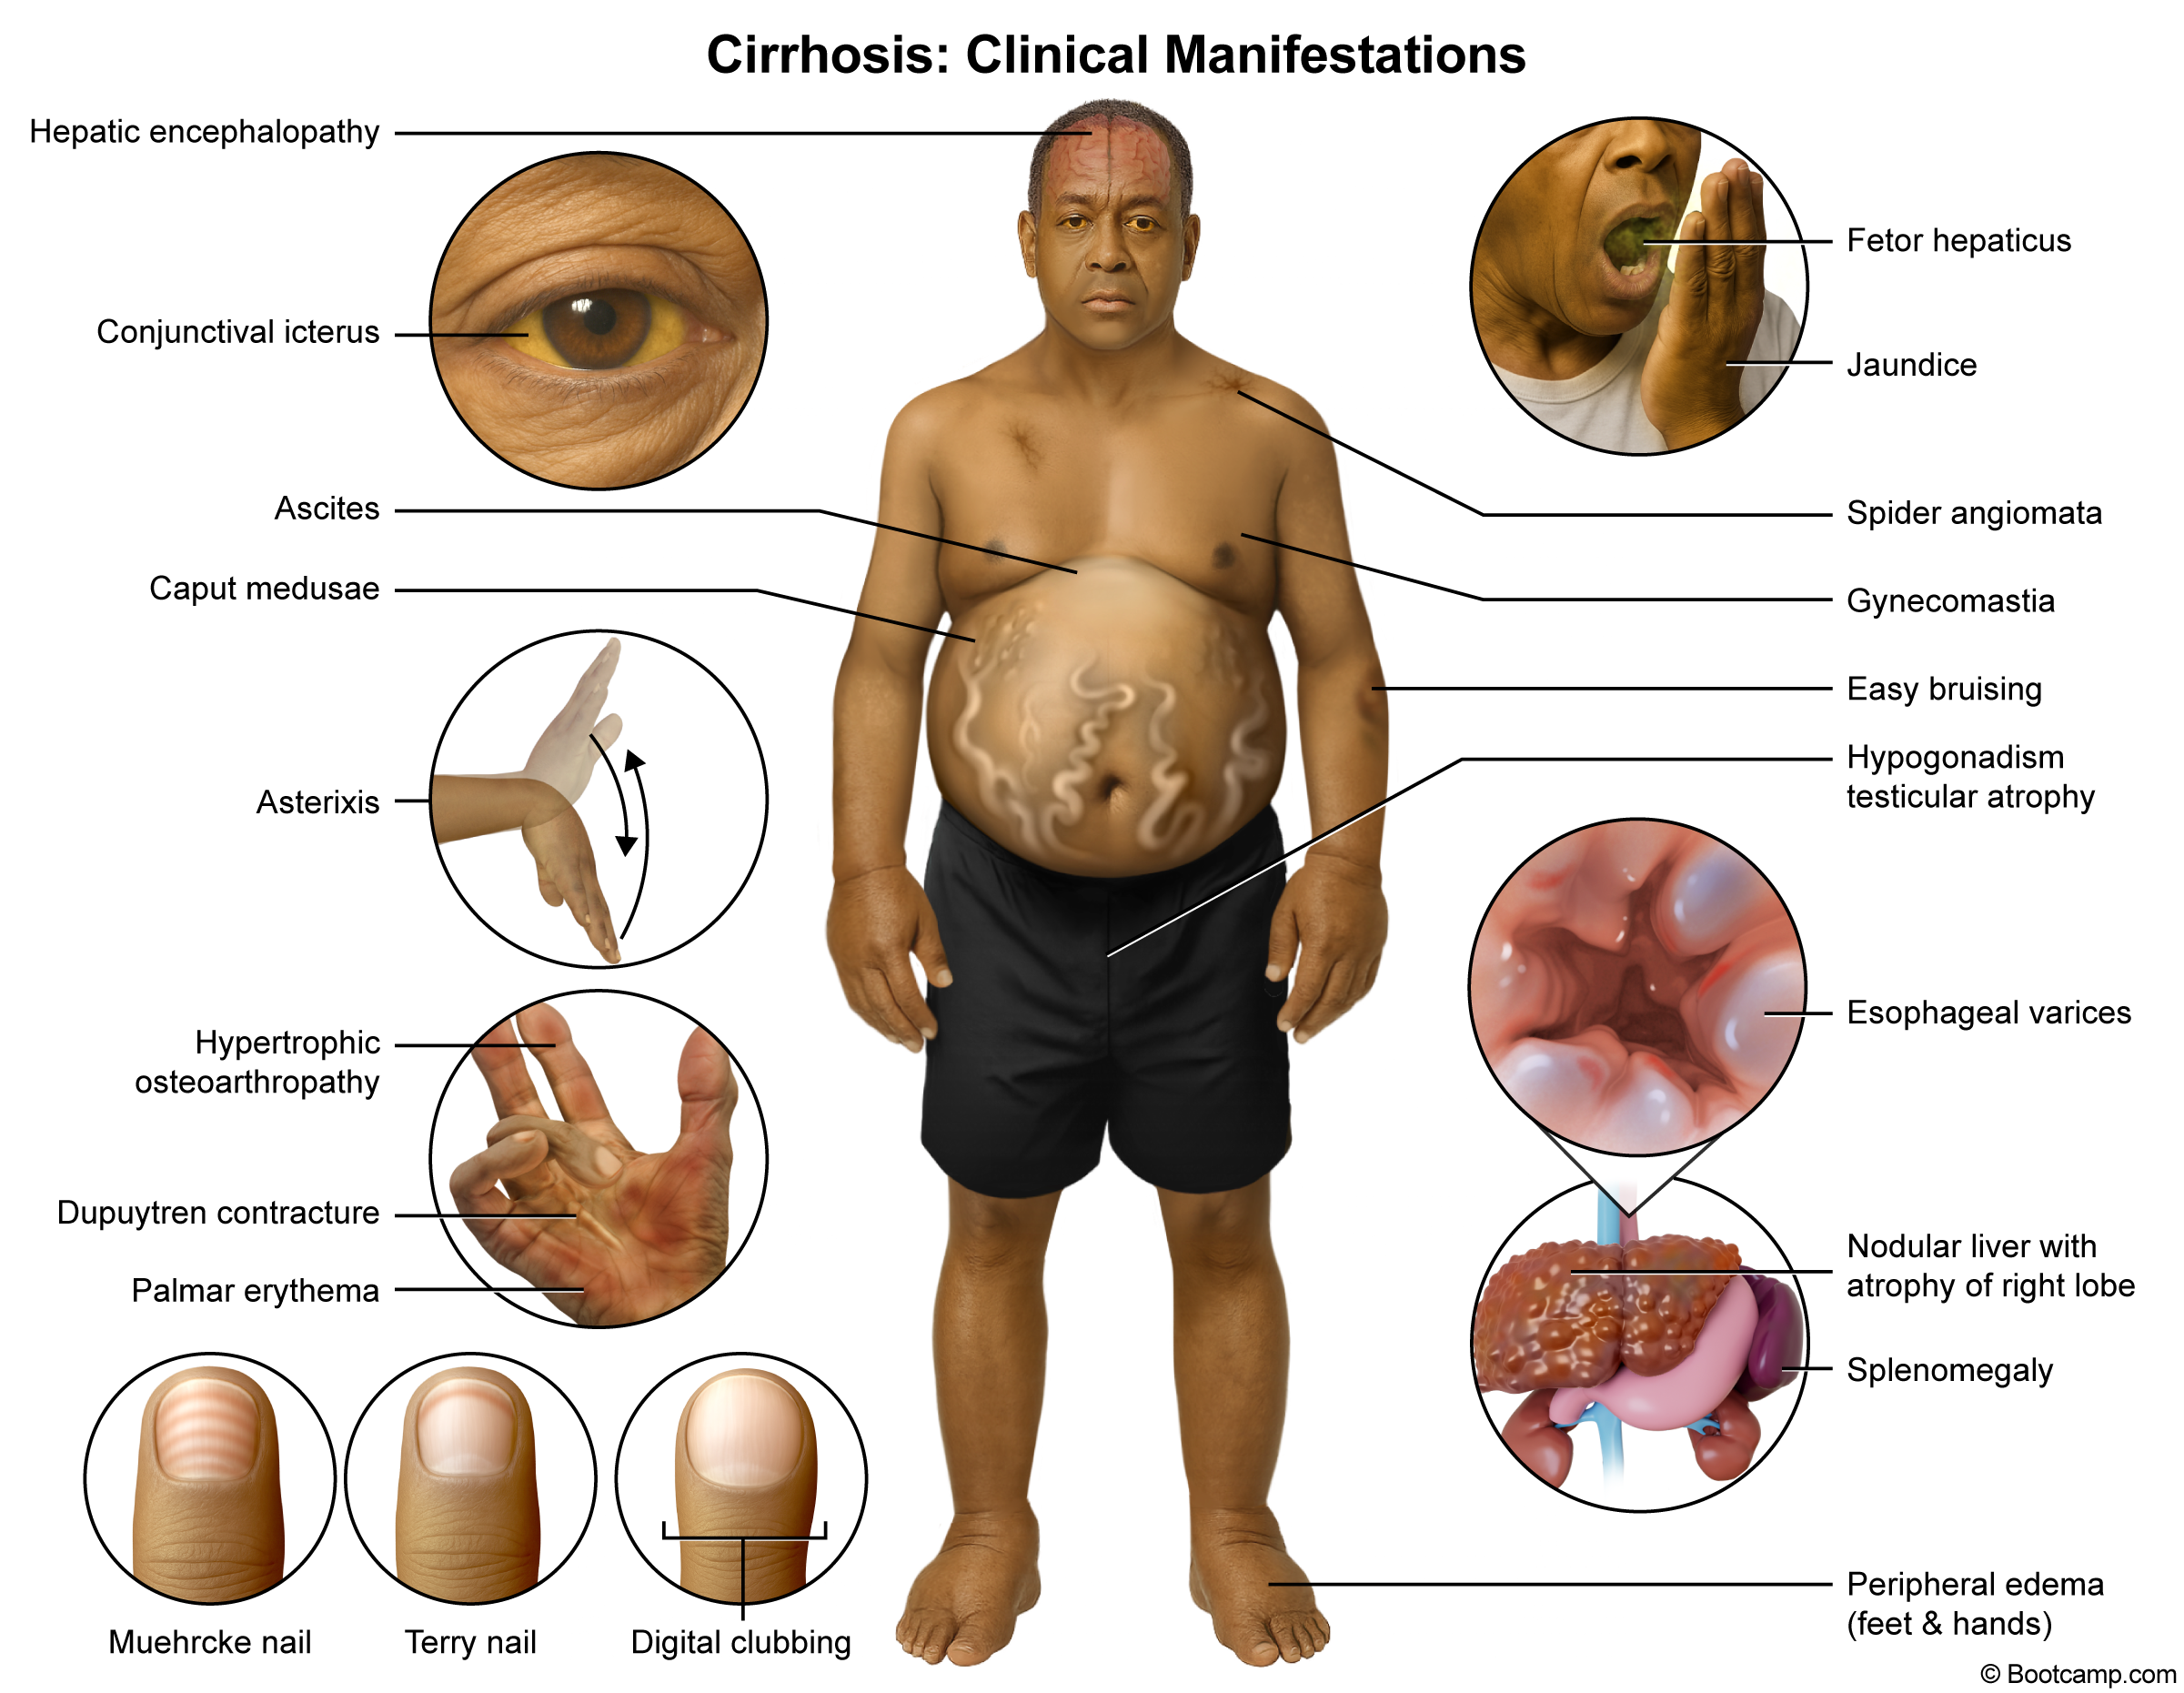
\includegraphics[keepaspectratio]{cld1.png}}

}

\caption{Stigmata of chronic liver disease - Bootcamp}

\end{figure}%

\section{WIPPER and the intro}\label{wipper-and-the-intro-3}

\begin{itemize}
\tightlist
\item[$\square$]
  Introduce yourself and shake hands
\item[$\square$]
  Washing of hands and appropriate hand hygiene
\item[$\square$]
  Asking for permission
\item[$\square$]
  Ensuring the room's privacy
\item[$\square$]
  Ensuring the environmental warmth and good lighting conditions
\item[$\square$]
  Asking for appropriate exposure (from the \textbf{xiphisternum} to the
  \textbf{symphysis pubis}) (nipples to mid thigh originally)
\item[$\square$]
  Asking the patient to be in the appropriate position (flat with \(1\)
  or \(2\) pillows \textasciitilde{} around \(10-15\) degrees)
\item[$\square$]
  Relocating to the right side of the patient
\item[$\square$]
  Asking for a chaperon
\item[$\square$]
  ``I have all of my equipment's''
\end{itemize}

\section{General look of the
patient}\label{general-look-of-the-patient-3}

\begin{itemize}
\tightlist
\item[$\square$]
  \textbf{Consciousness, alertness and orientation} of the patient to
  time, place and person (After asking
  \href{miscellaneous.qmd}{\emph{the} \(3\) questions)}
\item[$\square$]
  Comment on the patient's position and comfort
\item[$\square$]
  Comment on the patient's \textbf{external devices} status, such as
  \textasciitilde{} stomas, drains, catheters, etc
\item[$\square$]
  Patient is not in respiratory distress, not tachycardic, if he's
  cachectic or obese
\end{itemize}

\section{Vital signs}\label{vital-signs-3}

\begin{itemize}
\tightlist
\item[$\square$]
  Make sure you know the \href{miscellaneous.qmd}{\(6\) vital signs}
\item[$\square$]
  Take height and weight to calculate BMI and assess nutritional status
\end{itemize}

\section{Hands}\label{hands-1}

Starting with a quick glance at the nails:

\begin{itemize}
\tightlist
\item[$\square$]
  No \textbf{finger clubbing}
\item[$\square$]
  No \textbf{koilonychia} (\emph{IDA}), \textbf{leukonychia}
  (\emph{Hypoalbuminemia})
\end{itemize}

\emph{{[}Mention \textbf{Terry's Nails}, type of apparent leukonychia,
characterized by ground glass opacification of nearly the entire
nail{]}}

\begin{figure}[H]

{\centering \pandocbounded{\includegraphics[keepaspectratio]{cld2.png}}

}

\caption{Terry's Nails}

\end{figure}%

Moving to the still-hand examination:

\begin{itemize}
\tightlist
\item[$\square$]
  No \textbf{dupuytren's contracture} (Alcohol-related CLD)
\item[$\square$]
  No muscle wasting
\item[$\square$]
  No \textbf{palmar erythema}
\item[$\square$]
  No \textbf{Hypertrophic osteoarthropathy} (clubbing + periostitis of
  hand joints)
\item[$\square$]
  No marks of \textbf{I.V drug abuse}
\end{itemize}

Palpation + tests:

\begin{itemize}
\tightlist
\item[$\square$]
  Palpate temperature and dryness/sweatiness (bilaterally)
\item[$\square$]
  Test for \textbf{flapping tremor (Asterixis)} (don't apply
  resistance!)
\end{itemize}

\section{Face}\label{face-2}

\textbf{Eyes}

\begin{itemize}
\tightlist
\item[$\square$]
  Retract upper eyelid → no \textbf{jaundice}
\item[$\square$]
  Examine conjunctiva → no \textbf{pallor}
\end{itemize}

\textbf{Cheeks \& Lips}

\begin{itemize}
\tightlist
\item[$\square$]
  No \textbf{sialadenitis/sialadenosis} (parotid swelling; chronic
  alcohol abuse)
\item[$\square$]
  No \textbf{spider nevi} (better mentioned on chest)
\end{itemize}

\textbf{Mouth}

\begin{itemize}
\tightlist
\item[$\square$]
  No \textbf{halitosis} (\emph{Fetor hepaticus})
\end{itemize}

\section{Neck}\label{neck-1}

Nothing specific to CLD stigmata.

\section{Chest}\label{chest-1}

\begin{itemize}
\tightlist
\item[$\square$]
  Normal hair distribution (no \textbf{hair loss})
\item[$\square$]
  No \textbf{scratch marks}
\item[$\square$]
  No \textbf{spider nevi}
\item[$\square$]
  No \textbf{gynecomastia} (male) / \textbf{breast atrophy} (female)
\end{itemize}

\section{Abdominal Exam}\label{abdominal-exam-1}

\subsection{Inspection -- Foot of the
Bed}\label{inspection-foot-of-the-bed-1}

\begin{itemize}
\tightlist
\item[$\square$]
  \textbf{Contour} (flat, protuberant, scaphoid)\\
  \emph{In CLD → \textbf{distended abdomen} due to \textbf{ascites}}
\end{itemize}

\subsection{Inspection -- Right Side}\label{inspection-right-side}

\begin{itemize}
\tightlist
\item[$\square$]
  No distended veins (\textbf{Caput medusae})
\item[$\square$]
  No \textbf{bruising}
\end{itemize}

\subsection{Palpation \& Percussion}\label{palpation-percussion}

\textbf{Tips:}

\begin{itemize}
\tightlist
\item
  Palpate and percuss organs systematically with respiration.
\item
  Normal liver span: 6--12 cm.
\item
  Spleen → percuss ribs 9--11 (normally dull, non-ballottable).
\end{itemize}

\subsection{Liver -- Palpation}\label{liver-palpation-1}

\begin{itemize}
\tightlist
\item[$\square$]
  Start at RIF, move 1 cm at a time with inspiration/expiration.
\item[$\square$]
  If found → comment (smooth, sharp, non-tender edge).\\
\item[$\square$]
  If not found → percuss upwards.
\end{itemize}

\subsection{Liver -- Percussion}\label{liver-percussion-1}

\begin{itemize}
\tightlist
\item[$\square$]
  Ask for breath hold (after full expiration).
\item[$\square$]
  During expiration, percuss down from the 2nd intercostal space to the
  point of dullness.
\item[$\square$]
  Measure span (6--12 cm normal, \textbf{no hepatomegaly}).
\end{itemize}

\subsection{Spleen -- Palpation}\label{spleen-palpation-1}

\begin{itemize}
\tightlist
\item[$\square$]
  Start from RIF diagonally, normally impalpable.
\item[$\square$]
  Roll patient and palpate again from umbilicus.
\item[$\square$]
  Impalpable spleen; \textbf{no spleenomegaly}.
\end{itemize}

\subsection{Spleen -- Percussion}\label{spleen-percussion-1}

\begin{itemize}
\tightlist
\item[$\square$]
  Percuss ribs 9--11 → normal dullness.
\end{itemize}

\section{Ascites Assessment}\label{ascites-assessment-1}

Three tests:

\begin{enumerate}
\def\labelenumi{\arabic{enumi}.}
\tightlist
\item
  \textbf{Shifting dullness}

  \begin{itemize}
  \tightlist
  \item
    Percuss midline → flank dullness\\
  \item
    Roll patient (wait 15s) → \textbf{no shifting dullness}
  \end{itemize}
\item
  \textbf{Fluid thrill}

  \begin{itemize}
  \tightlist
  \item
    Hand on midline, flick other side\\
  \item
    \textbf{No transmitted thrill}
  \end{itemize}
\item
  \textbf{Succussional splash} (mention only)
\end{enumerate}

\section{Auscultation}\label{auscultation-2}

\begin{itemize}
\tightlist
\item[$\square$]
  Auscultate over liver, spleen\\
\item[$\square$]
  No friction rub
\end{itemize}

\section{Ending the Station}\label{ending-the-station-3}

\begin{itemize}
\tightlist
\item[$\square$]
  Examine \textbf{external genitalia} \emph{(atrophy)}\\
\item[$\square$]
  Examine \textbf{PR (anorectal varices)}\\
\item[$\square$]
  Examine \textbf{lower limb for edema, hair loss}\\
\item[$\square$]
  Check \textbf{sacral edema}
\end{itemize}

\subsection{Hepatic Encephalopathy}\label{hepatic-encephalopathy}

We assess grade using \textbf{West Haven Criteria}:

\begin{figure}[H]

{\centering \pandocbounded{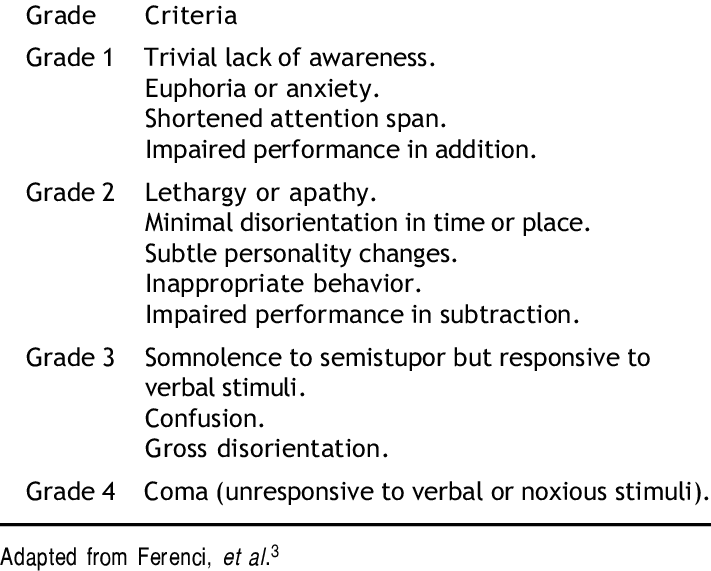
\includegraphics[keepaspectratio]{cld3.png}}

}

\caption{West Haven Hepatic Encephalopathy Grading}

\end{figure}%

THE END

\bookmarksetup{startatroot}

\chapter{Thyroid checklist}\label{thyroid-checklist}

\begin{figure}[H]

{\centering \pandocbounded{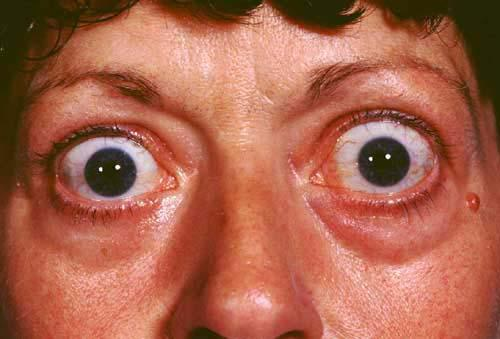
\includegraphics[keepaspectratio]{thyroid1.png}}

}

\caption{Graves' ophthalmopathy}

\end{figure}%

\section{WIPPER and the intro}\label{wipper-and-the-intro-4}

\begin{itemize}
\tightlist
\item[$\square$]
  Introduce yourself and shake hands
\item[$\square$]
  Washing of hands and appropriate hand hygiene
\item[$\square$]
  Asking for permission
\item[$\square$]
  Ensuring the room's privacy
\item[$\square$]
  Ensuring the environmental warmth and good lighting conditions
\item[$\square$]
  Asking for appropriate exposure (\textbf{The neck and the upper
  chest})
\item[$\square$]
  Asking the patient to be in the appropriate position
  (\textbf{Sitting})
\item[$\square$]
  Relocating to the right side of the patient
\item[$\square$]
  Asking for a chaperon
\item[$\square$]
  ``I have all of my equipment's''
\end{itemize}

\section{General look of the
patient}\label{general-look-of-the-patient-4}

\begin{itemize}
\tightlist
\item[$\square$]
  \textbf{Consciousness, alertness and orientation} of the patient to
  time, place and person (After asking the \href{miscellaneous.qmd}{3
  questions})
\item[$\square$]
  Comment on the patient's position and \textbf{comfort}
\item[$\square$]
  Patient is \textbf{not in distress, tachypnea or in pain, not obese
  nor thin}
\item[$\square$]
  Comment that the patient is showing \textbf{normal facial expression,
  no apathy or agitation}
\item[$\square$]
  Ask the patient to \textbf{say his full name}
\item[$\square$]
  Comment on the patient's \textbf{normal clothing for the weather}
\item[$\square$]
  Comment on \textbf{normal speech with no hoarseness, no slow or
  pressured speech}
\end{itemize}

\section{Vital signs}\label{vital-signs-4}

\begin{itemize}
\tightlist
\item[$\square$]
  Mention that you want to check the pulse as \textbf{tachycardia} and
  \textbf{atrial fibrillation} occur with \textbf{hyperthyroidism} and
  \textbf{bradycardia} with \textbf{hypothyroidism}
\item[$\square$]
  Mention that you will have to check the blood pressure for
  \textbf{diastolic/systolic HTN}
\item[$\square$]
  Mention that you will have to check the \textbf{BMI for weight
  gain/loss}
\item[$\square$]
  you might be asked to mention the \href{miscellaneous.qmd}{rest of the
  vital signs}
\end{itemize}

\section{Hands}\label{hands-2}

\textbf{Inspect for; palm and dorsum}

\begin{itemize}
\tightlist
\item[$\square$]
  No \textbf{palmar erythema}
\item[$\square$]
  No \textbf{thenar/hypothenar muscle wasting}
\item[$\square$]
  No \textbf{vitiligo}
\item[$\square$]
  Normal \textbf{hair distribution}
\item[$\square$]
  No \textbf{dry and course skin}
\end{itemize}

\textbf{Nail changes;}

\begin{itemize}
\tightlist
\item[$\square$]
  No \textbf{finger clubbing}
\item[$\square$]
  No \textbf{onycholysis}
\item[$\square$]
  No \textbf{thyroid acropachy}
\item[$\square$]
  No \textbf{brittle nails}
\item[$\square$]
  Do the \href{miscellaneous.qmd}{usuals for palpation}, check and
  comment on \textbf{hand's temperature, dryness/sweatiness}
\end{itemize}

\textbf{Tests;}

\begin{itemize}
\tightlist
\item[$\square$]
  Ask the patient to extend his arms (يمد ايديه)
\item[$\square$]
  Comment on no \textbf{fine tremor}
\item[$\square$]
  Do the \textbf{carpal tunnel test}! (You can find it
  \href{mss.qmd}{here} in the mss checklist)
\end{itemize}

\bookmarksetup{startatroot}

\chapter{Face}\label{face-3}

\begin{itemize}
\tightlist
\item[$\square$]
  No \textbf{dry or coarse hair, no hair loss}
\item[$\square$]
  No \textbf{hair loss of last third of eyebrows}
  (\emph{Hypothyroidism})
\item[$\square$]
  No \textbf{periorbital puffiness or myxedema}
\item[$\square$]
  No \textbf{lid retraction}
\item[$\square$]
  Ask the patient to look at your finger without moving his head, test
  for lid lag (vertically move your finger)
\item[$\square$]
  No \textbf{lid lag}
\item[$\square$]
  No \textbf{exophthalmos}
\item[$\square$]
  No \textbf{proptosis}
\item[$\square$]
  No \textbf{Conjunctival redness} (Chemosis)
\item[$\square$]
  Test for \textbf{Ophthalmoplegia} (H shape)!
\item[$\square$]
  Comment on \textbf{no diplopia or nystagmus}
\end{itemize}

\section{Thyroid}\label{thyroid}

\subsection{Inspection}\label{inspection-2}

\begin{itemize}
\tightlist
\item[$\square$]
  Ask the patient to \textbf{hyperextend his neck}, look at his thyroid
\item[$\square$]
  No \textbf{scars, swellings, skin lesions}
\item[$\square$]
  No \textbf{asymmetry}
\item[$\square$]
  No \textbf{visible dilated veins}
\item[$\square$]
  Ask the patient to swallow
\item[$\square$]
  Mention that \textbf{thyroid moves with swallowing}
\item[$\square$]
  Ask the patient to protrude his tongue
\item[$\square$]
  Mention that \textbf{thyroid doesn't move} (\emph{No thyroglossal
  cyst})
\item[$\square$]
  Ask the patient to raise his arms, notice any facial congestions
  (\textbf{Pemberton's sign})
\item[$\square$]
  Comment \textbf{negative Pemberton's sign}
\end{itemize}

\subsection{Palpation}\label{palpation-3}

\begin{itemize}
\tightlist
\item[$\square$]
  As always, do the \href{miscellaneous.qmd}{usuals before palpation}
\item[$\square$]
  Stand behind the patient, ask him to slightly look down (Neck flexion)
\item[$\square$]
  Palpate the thyroid
\item[$\square$]
  Comment on \textbf{symmetrical thyroid lobes}
\item[$\square$]
  Comment on \textbf{no tenderness} (Make sure to hold eye contact to
  notice any tenderness)
\item[$\square$]
  Comment on \textbf{no nodules or masses}
\item[$\square$]
  Comment on \textbf{no enlargement}
\item[$\square$]
  Feel for thrills, comment on \textbf{no thrills}
\item[$\square$]
  Mention \textbf{palpating cervical lymph nodes}! (should be skipped)
\item[$\square$]
  Ask the patient to swallow, comment on \textbf{thyroid moves while
  swallowing}
\item[$\square$]
  Ask the patient to protrude his tongue, comment on \textbf{no
  movement}
\end{itemize}

\subsection{Tracheal tests}\label{tracheal-tests}

\begin{itemize}
\tightlist
\item[$\square$]
  Using 3 fingers, check for \textbf{tracheal deviation} (comment that
  it's centralized)
\item[$\square$]
  Ask the patient to take a deep inspiration, to check for tracheal tug
\item[$\square$]
  Comment on \textbf{no tracheal tug}
\item[$\square$]
  Measure the \textbf{crico-sternal distance} (Normally; 3 to 4 fingers)
\end{itemize}

\subsection{Percussion}\label{percussion}

\begin{itemize}
\tightlist
\item[$\square$]
  Percuss over the \textbf{clavicle's head}, note if there's dullness
\end{itemize}

\emph{dullness = retrosternal goiter}

\begin{itemize}
\tightlist
\item[$\square$]
  Comment on \textbf{no dullness, normal resonance}
\item[$\square$]
  Percuss over the \textbf{manubrium} too, and comment \textbf{no
  dullness, normal resonance}
\end{itemize}

\subsection{Auscultation}\label{auscultation-3}

\begin{itemize}
\tightlist
\item[$\square$]
  Auscultate for \textbf{thyroid bruit}
\item[$\square$]
  Mention no thyroid bruit
\item[$\square$]
  Auscultate for murmurs
\item[$\square$]
  Mention** no midsystolic murmur**
\end{itemize}

\section{Finishing off your station!}\label{finishing-off-your-station}

I want to check/examine for;

\begin{itemize}
\tightlist
\item[$\square$]
  \textbf{Proximal myopathy} (Testing for it would be by asking the
  patient to stand up with his hands on his chest
\item[$\square$]
  Test for \textbf{deep tendon reflexes} \emph{(in hypothyroidism =
  \textbf{delayed relaxation}, in hyperthyroidism =
  \textbf{hyperreflexia})}
\item[$\square$]
  \textbf{Pretibial myxedema} of \emph{grave's}
\item[$\square$]
  \textbf{Ankle swelling} of heart failure
\item[$\square$]
  \textbf{Lower limb skin} if its \emph{dry and coarse}
\end{itemize}

THE END

\bookmarksetup{startatroot}

\chapter{Hand and Wrist checklist}\label{hand-and-wrist-checklist}

\section{Rules:}\label{rules}

\begin{enumerate}
\def\labelenumi{\arabic{enumi}.}
\tightlist
\item
  Look, feel and move :)
\item
  We don't say abnormal until we compare right and left!
\end{enumerate}

\section{WIPPER and the intro}\label{wipper-and-the-intro-5}

\begin{itemize}
\tightlist
\item[$\square$]
  Introduce yourself and shake hands
\item[$\square$]
  Washing of hands and appropriate hand hygiene
\item[$\square$]
  Asking for permission
\item[$\square$]
  Ensuring the room's privacy
\item[$\square$]
  Ensuring the environmental warmth and good lighting conditions
\item[$\square$]
  Asking for appropriate exposure (\textbf{One joint above, one joint
  below})
\item[$\square$]
  Asking the patient to be in the appropriate position (\textbf{Sitting
  upright with a pillow under his hands})
\item[$\square$]
  Relocating to the right side of the patient
\item[$\square$]
  Asking for a chaperon
\item[$\square$]
  ``I have all of my equipment's''
\end{itemize}

\section{Vital signs:}\label{vital-signs-5}

\begin{itemize}
\tightlist
\item[$\square$]
  Make sure you know the \href{miscellaneous.qmd}{6 vital signs}
\end{itemize}

\bookmarksetup{startatroot}

\chapter{Look}\label{look}

Look at the palm, dorsum, lateral sides of the hands and in between
fingers.

\begin{itemize}
\tightlist
\item[$\square$]
  No \textbf{scars, skin rash, no bruises} :)
\item[$\square$]
  No \textbf{color changes}; \textbf{palmar erythema}, (\emph{raynaud's
  syndrome})
\item[$\square$]
  No \textbf{nail changes}; \textbf{nail pitting/brittle nails} \ldots{}
\item[$\square$]
  No \textbf{deformities}; Swan neck / boutonnière/ mallet / Trigger
  finger / Sausage fingers / dupuytren's contractures
  (\emph{Alcoholic-CLD}) / Z thumb (\emph{RA}) / Ulnar deviation
  (\emph{RA})
\item[$\square$]
  No \textbf{skin nodules} \textasciitilde{} Bouchard's/Heberden's
  (\emph{Osteoarthritis})
\item[$\square$]
  No \textbf{gouty tophi}
\item[$\square$]
  No \textbf{visible soft tissue swelling}
\item[$\square$]
  No \textbf{muscle wasting} (thenar wasting in carpal tunnel syndrome)/
  \textbf{hypertrophy} / \textbf{fasciculations}
\item[$\square$]
  While looking at the hand's fingertips, mention \textbf{No Calcinosis}
  (\emph{Systemic Sclerosis})
\item[$\square$]
  Ask the patient to form a fist, mention \textbf{No loss of
  ``Hill-Valley-Hill-Valley''} on the dorsal aspect of the hand
  (\emph{RA})
\end{itemize}

Look at the patient's elbow

\begin{itemize}
\tightlist
\item[$\square$]
  Comment on ``No \emph{rheumatoid} nodules''
\end{itemize}

\bookmarksetup{startatroot}

\chapter{Feel}\label{feel}

\begin{itemize}
\tightlist
\item[$\square$]
  Palpate dorsum of the hand to check for \textbf{temperature/dryness
  and sweatiness} (and comment)
\item[$\square$]
  \textbf{Pinch the skin} of the dorsal aspect of the hand, mention
  \textbf{No thick nor tightening} of the skin found
  (\emph{Scleroderma-Rodnan score})
\end{itemize}

\begin{figure}[H]

{\centering 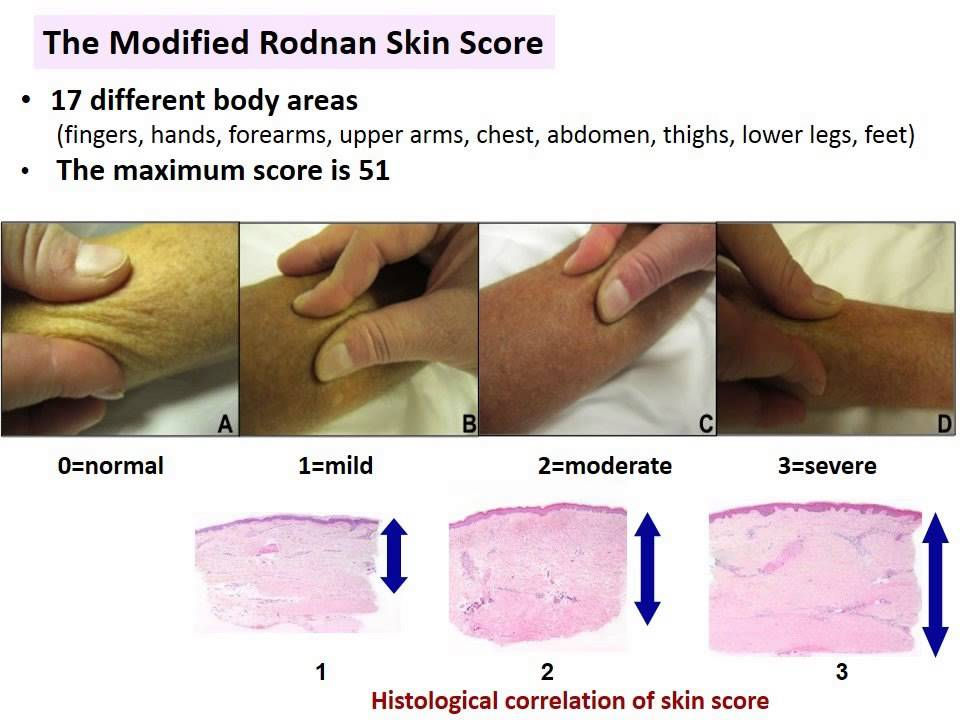
\includegraphics[width=5.20833in,height=3.125in]{mss10.png}

}

\caption{Scleroderma-Rodnan Score}

\end{figure}%

\begin{itemize}
\tightlist
\item[$\square$]
  Check all other joints for \textbf{soft tissue swelling and
  fluctuations} using your 2 thumbs (Wrist joint, MCP, PIP, DIP, don't
  forget the thumb's 2 joints!)
\item[$\square$]
  \textbf{Squeeze test} \textasciitilde{} squeeze all MCP joints for
  \textbf{tenderness}
\end{itemize}

\bookmarksetup{startatroot}

\chapter{Move}\label{move}

\begin{itemize}
\tightlist
\item[$\square$]
  Give the patient 2 fingers and ask him to \textbf{squeeze to assess
  power} of his hands
\item[$\square$]
  Comment on normal power
\item[$\square$]
  Ask the patient to move his \textbf{wrist in all 4 directions} to
  assess range of motion in his wrist
\item[$\square$]
  Comment on full range of motion
\item[$\square$]
  Ask the patient to move his \textbf{thumb in all directions} to assess
  its range of motion, and ask him to move it against resistance too.
\item[$\square$]
  Ask the patient to count their fingers (\textbf{MCP joint flexion
  maneuver})
\item[$\square$]
  Test \textbf{flexor digitorum profundus} (isolate each finger, and ask
  to do flexion on \textbf{DIP} (extend pip)) and \textbf{flexor
  digitorum superficialis} (isolate each finger, and ask to do flexion
  on \textbf{PIP} (extend MCP))
\item[$\square$]
  Ask the patient to form a semi fist and make sure his fingers point
  towards \textbf{scaphoid bone}
\item[$\square$]
  \textbf{Finkelstein's test}; ask the patient to make fist with thumb
  tucked inside, then ask him to do ulnar deviation. Positive test: pain
  above the radial side of the hand. \emph{De Quervain's tenosynovitis}
  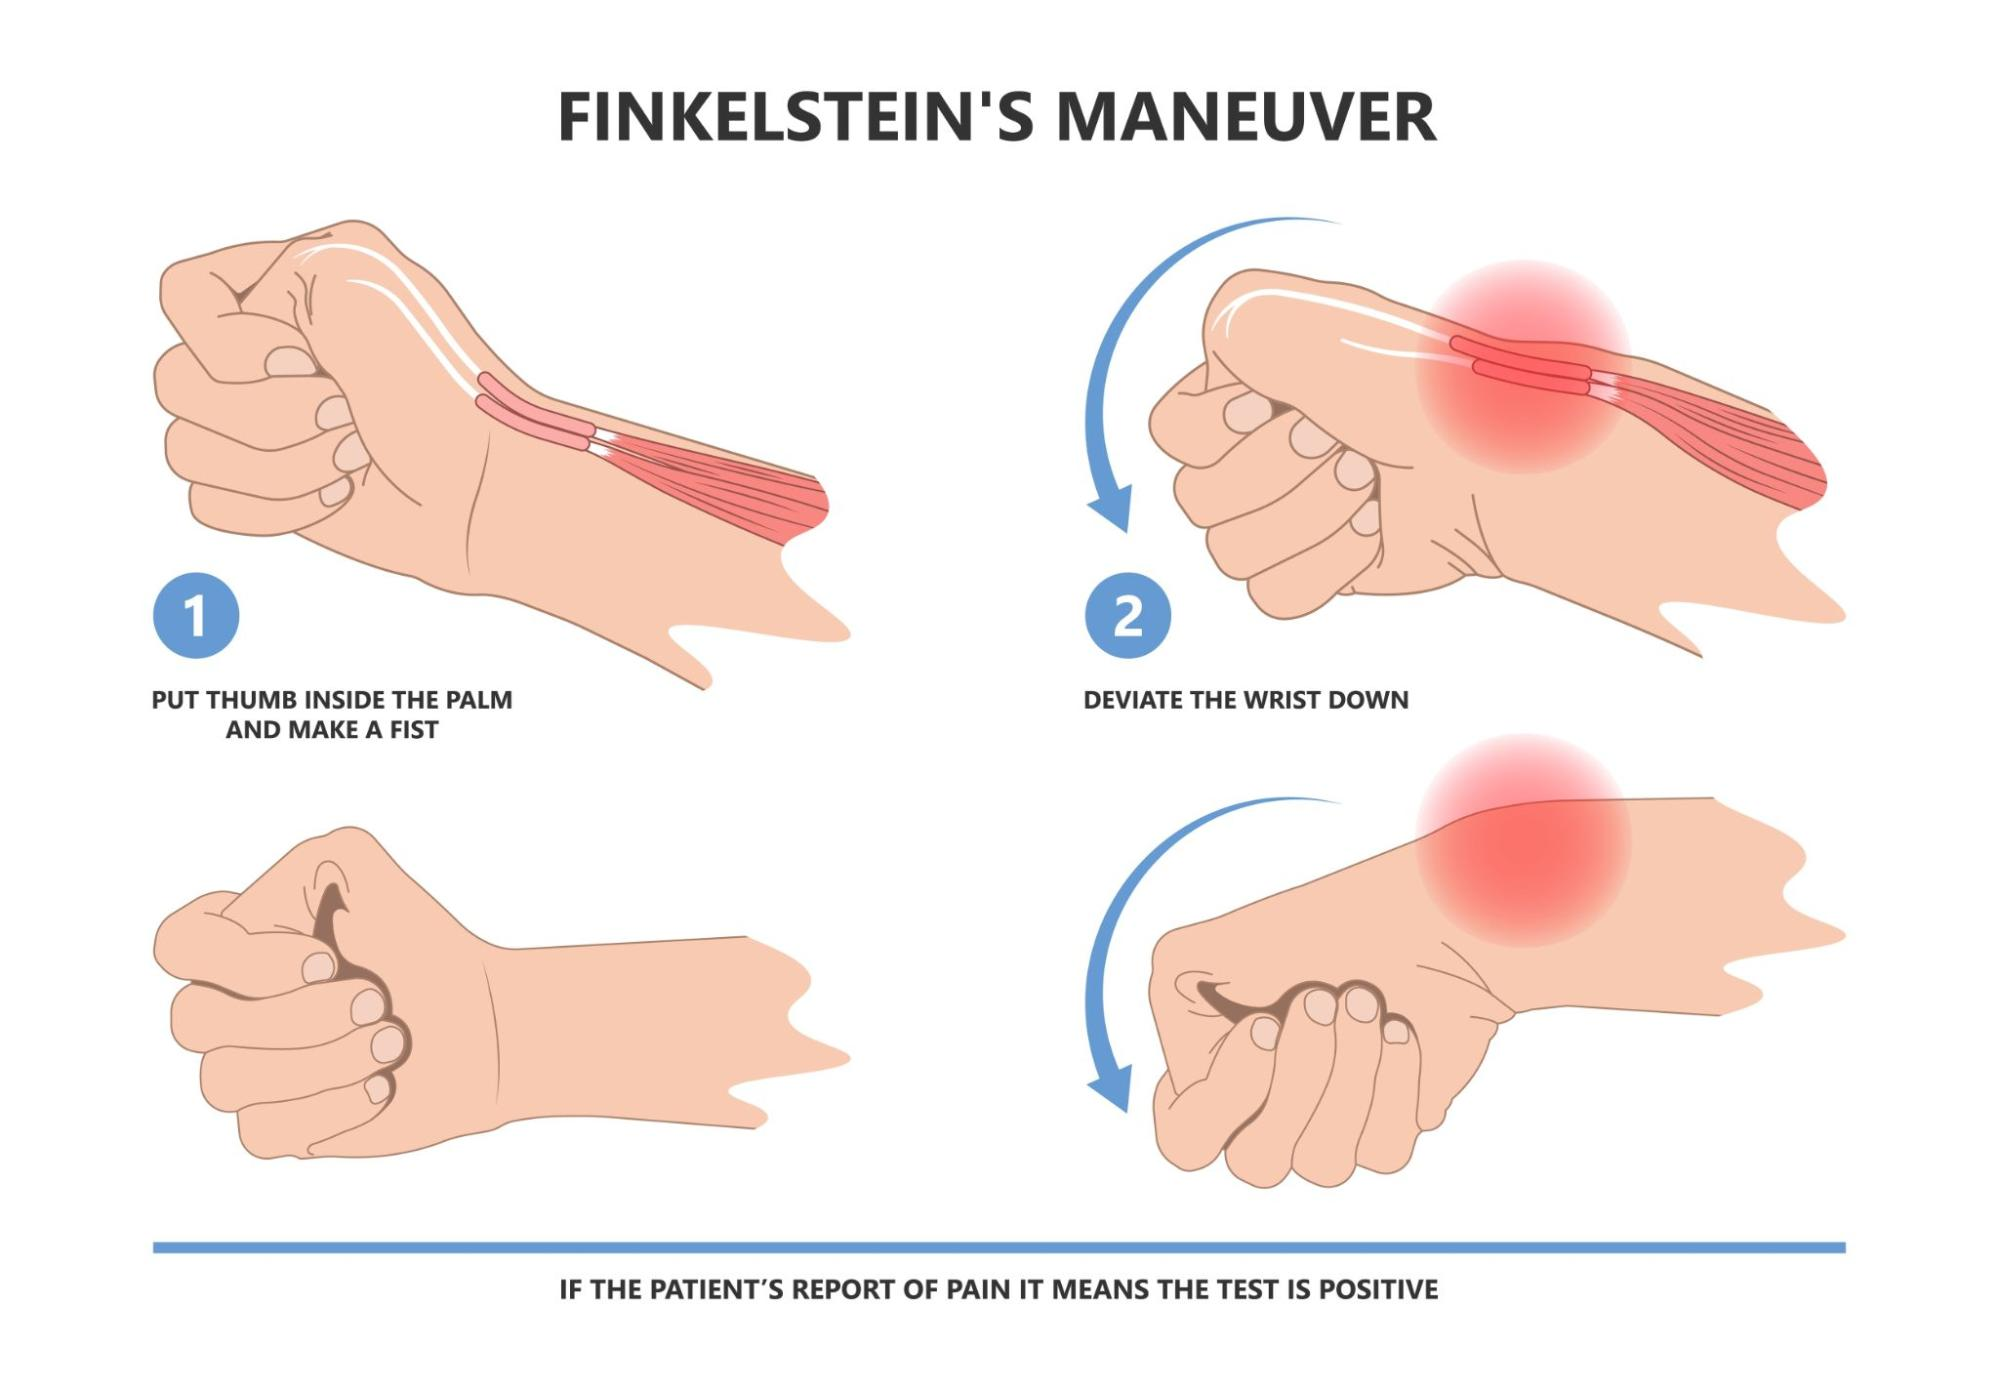
\includegraphics[width=5.20833in,height=3.48958in]{mss0.png}
\end{itemize}

\subsection{Nerves}\label{nerves}

\subsection{Median nerve}\label{median-nerve}

\begin{itemize}
\tightlist
\item[$\square$]
  For motor, ask the patient to do ``\textbf{Ok sign}'' this is only
  testing the anterior interosseous branch of median, that's why we need
  a test for median proper, next step for that.
\item[$\square$]
  After patient does the ``Ok sign'', assess its power by trying to pull
  on his ok sign after asking him to resist.
\end{itemize}

\begin{figure}[H]

{\centering 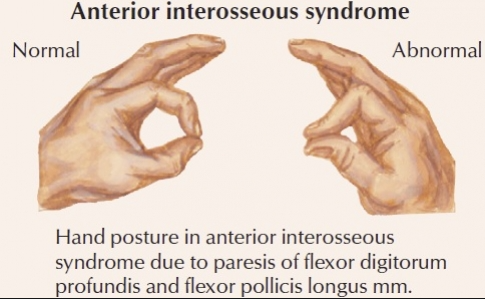
\includegraphics[width=5.20833in,height=3.125in]{mss1.png}

}

\caption{Ok sign and anterior interosseous syndrome}

\end{figure}%

\begin{itemize}
\tightlist
\item[$\square$]
  To test median nerve proper, we do opposition test of thumb (Oppose
  thumb and little finger)
\item[$\square$]
  For sensory, ask the pt to close his eyes, palpate thenar eminence and
  ask if patient felt it.
\end{itemize}

\subsection{Ulnar nerve}\label{ulnar-nerve}

\begin{itemize}
\tightlist
\item[$\square$]
  For motor, ask the patient to \textbf{abduct and adduct his fingers
  (scissoring)}. Also,\\
  Adduction power can be assessed by putting a paper between patient's
  finger (Ask him to not let it go) and trying to pull it.\\
  Abduction power can be assessed by:
\end{itemize}

Ulnar - abduction testing

Scissoring

\begin{itemize}
\tightlist
\item[$\square$]
  For sensory, ask the pt to close his eyes, palpate hypothenar eminence
  and ask if patient felt it
\end{itemize}

\subsection{Radial nerve}\label{radial-nerve}

\begin{itemize}
\tightlist
\item[$\square$]
  For \textbf{motor}, ask the patient to \textbf{extend his fingers at
  (MCP joint)} ask the patient to lay hand flat on a table, and raise
  only the fingers. (Then against resistance for power assessment)
\end{itemize}

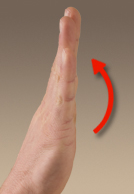
\includegraphics[width=2.08333in,height=3.125in]{mss4.png}

\begin{itemize}
\tightlist
\item[$\square$]
  For \textbf{sensory}, ask the pt to close his eyes, palpate dorsum of
  the hand on the lateral half
\end{itemize}

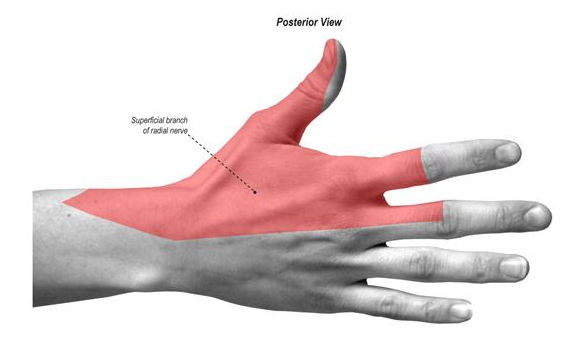
\includegraphics[width=5.20833in,height=3.125in]{mss5.png}

\textbf{Carpal tunnel syndrome} (3 tests);

\begin{enumerate}
\def\labelenumi{\arabic{enumi})}
\item
  \textbf{\emph{Carpal Compression Test (most sensitive)}}; compress
  with your thumb the position of the median nerve (Proximal to the
  distal hand crease) for 1 minute, this should (If the nerve is
  compressed) trigger the compression thus causing signs of carpal
  tunnel syndrome (Pain, Paresthesia and Numbness on the lateral 3.5
  fingers) aka \textbf{Durkan's test}
\item
  \textbf{Tinel's test}; tap the position of the median nerve (Proximal
  to the distal hand crease) for 1 minute, this should (If the nerve is
  compressed) trigger the compression thus causing signs of carpal
  tunnel syndrome (Pain, Paresthesia and Numbness on the lateral 3.5
  fingers)
\end{enumerate}

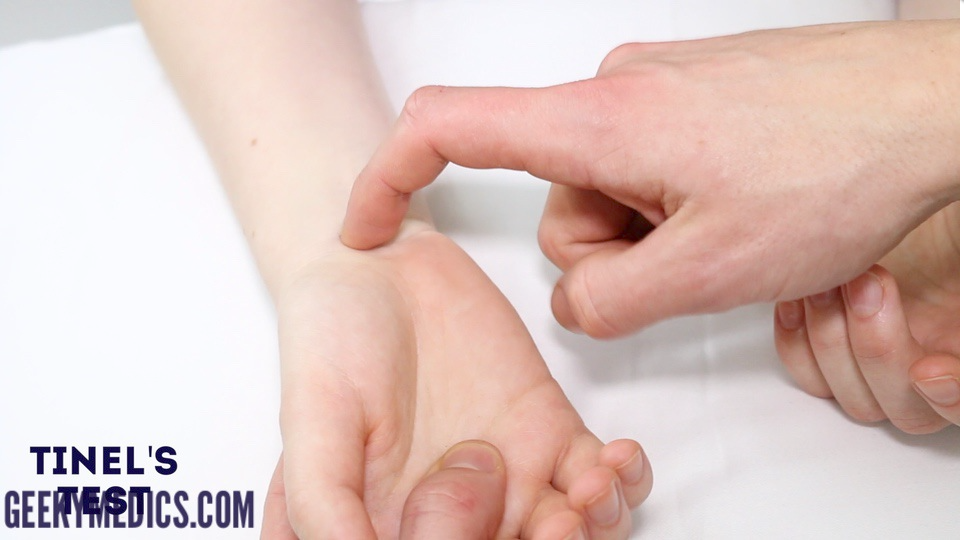
\includegraphics[width=5.20833in,height=3.125in]{mss6.png}

\begin{enumerate}
\def\labelenumi{\arabic{enumi})}
\setcounter{enumi}{2}
\tightlist
\item
  \textbf{Phalen's test}; (Reverse prayer) for 1 minute, a positive test
  again will produce symptoms of carpal tunnel syndrome (Pain,
  Paresthesia and Numbness on the lateral 3.5 fingers)
\end{enumerate}

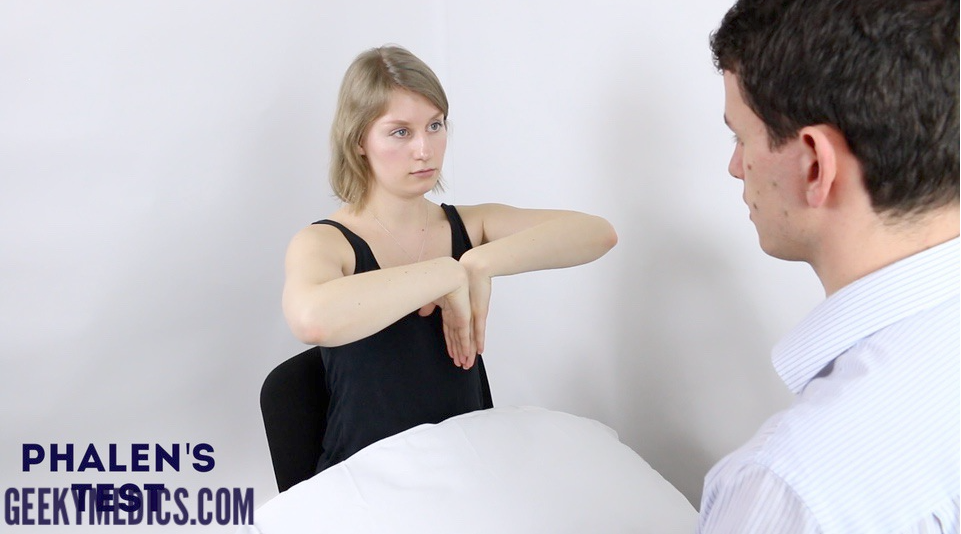
\includegraphics[width=5.20833in,height=3.125in]{mss7.png}

End your exam by:

\begin{itemize}
\tightlist
\item[$\square$]
  Mention doing a neurovascular check
\item[$\square$]
  Mention doing capilaary refill test
\item[$\square$]
  Mention assessing radial pulse
\end{itemize}

\bookmarksetup{startatroot}

\chapter{Peripheral Arterial Disease
checklist}\label{peripheral-arterial-disease-checklist}

\section{WIPPER and the Intro}\label{wipper-and-the-intro-6}

\begin{itemize}
\tightlist
\item[$\square$]
  Introduce yourself and shake hands\\
\item[$\square$]
  Washing of hands and appropriate hand hygiene\\
\item[$\square$]
  Asking for permission\\
\item[$\square$]
  Ensuring the room's privacy\\
\item[$\square$]
  Ensuring the environmental warmth and good lighting conditions\\
\item[$\square$]
  Asking for appropriate exposure (\textbf{from the waist and above and
  from the knees and down})\\
\item[$\square$]
  Asking the patient to be in the appropriate position
  (\textbf{semi-sitting at 45 degrees in bed})\\
\item[$\square$]
  Relocating to the right side of the patient\\
\item[$\square$]
  Asking for a chaperon\\
\item[$\square$]
  ``I have all of my equipment's''
\end{itemize}

\section{General Look of the
Patient}\label{general-look-of-the-patient-5}

\begin{itemize}
\tightlist
\item[$\square$]
  \textbf{Consciousness, alertness and orientation} of the patient to
  time, place and person (\href{miscellaneous.qmd}{After asking the 3
  questions})\\
\item[$\square$]
  Comment on the patient's \textbf{position and comfort}\\
\item[$\square$]
  Comment on no obvious \textbf{shortness of breath} (PE)\\
\item[$\square$]
  Comment on the patient's \textbf{external devices} such as any
  mobility aids (Wheelchairs, walking aids)\\
\item[$\square$]
  Comment on any \textbf{Medical equipment's} such as any dressings or
  limb prosthesis\\
\item[$\square$]
  Comment on \textbf{cyanosis}\\
\item[$\square$]
  Comment on no \textbf{limb pallor}
\end{itemize}

\section{Vital Signs (Mention)}\label{vital-signs-mention}

\begin{itemize}
\tightlist
\item[$\square$]
  Mention measuring Blood pressure \textbf{bilaterally}\\
\item[$\square$]
  Make sure you know the \href{miscellaneous.qmd}{6 vital signs}
\end{itemize}

\section{Inspection}\label{inspection-3}

\begin{itemize}
\tightlist
\item[$\square$]
  Inspect the \textbf{upper} limbs bilaterally and do not forget the
  hands and fingers\\
\item[$\square$]
  Inspect the \textbf{lower} limbs bilaterally and do not forget the
  feet and toes, also check the back of the legs + sole\\
\item[$\square$]
  Mention no \textbf{missing limbs or digits, and no scars and no
  dressings}\\
\item[$\square$]
  Mention no \textbf{xanthomata} (\emph{Hyperlipidema is a major risk
  factor for PAD})\\
\item[$\square$]
  Mention no \textbf{Tar stain} (\emph{Smoking is a major risk factor
  for PAD})\\
\item[$\square$]
  Mention no \textbf{muscle wasting}\\
\item[$\square$]
  Mention seeing no \textbf{dry skin, no shiny skin, no hair loss, no
  thickened or brittle nails}\\
\item[$\square$]
  Mention no \textbf{signs of infections} such as fungal → \emph{between
  the toes}\\
\item[$\square$]
  Mention no \textbf{color changes} such as pallor or darker pigmented
  skin (\emph{Lipo-dermato-sclerosis})\\
\item[$\square$]
  Mention no \textbf{gangrene}
\end{itemize}

\begin{tcolorbox}[enhanced jigsaw, left=2mm, toptitle=1mm, breakable, title=\textcolor{quarto-callout-note-color}{\faInfo}\hspace{0.5em}{Note}, coltitle=black, opacitybacktitle=0.6, arc=.35mm, colback=white, leftrule=.75mm, toprule=.15mm, bottomtitle=1mm, titlerule=0mm, rightrule=.15mm, colbacktitle=quarto-callout-note-color!10!white, bottomrule=.15mm, opacityback=0, colframe=quarto-callout-note-color-frame]

\textbf{Gangrene definition}\\
Gross description of a necrotic tissue with mummification and black
discoloration.\\
Wet gangrene is infected, looks black and unclearly demarcated, needs
emergent amputation for risk of sepsis.\\
Dry gangrene is not infected, dark and well demarcated.\\
\emph{Finger tip necrosis is a sign for Buerger's disease aka
thromboangiitis obliterans.}

\end{tcolorbox}

\begin{itemize}
\tightlist
\item[$\square$]
  Mention no \textbf{ulcers}\\
\item[$\square$]
  Mention no \textbf{guttering of veins}
\end{itemize}

\begin{tcolorbox}[enhanced jigsaw, left=2mm, toptitle=1mm, breakable, title=\textcolor{quarto-callout-note-color}{\faInfo}\hspace{0.5em}{Note}, coltitle=black, opacitybacktitle=0.6, arc=.35mm, colback=white, leftrule=.75mm, toprule=.15mm, bottomtitle=1mm, titlerule=0mm, rightrule=.15mm, colbacktitle=quarto-callout-note-color!10!white, bottomrule=.15mm, opacityback=0, colframe=quarto-callout-note-color-frame]

\textbf{Guttering of veins}\\
In a warm room the veins of a normal foot are dilated and full of blood,
even when the patient is lying horizontally.\\
In an ischaemic foot the veins collapse and sink below the skin surface
to look like pale-blue gutters.

\end{tcolorbox}

\begin{itemize}
\tightlist
\item[$\square$]
  Ask the patient to move his limbs and mention no \textbf{paralysis}
\end{itemize}

\section{Palpation}\label{palpation-4}

\begin{itemize}
\tightlist
\item[$\square$]
  Do the \href{miscellaneous.qmd}{usuals for palpation}\\
\item[$\square$]
  Generally and gently palpate the limbs for any \textbf{tenderness or
  crepitus} (Gas gangrene)\\
\item[$\square$]
  Mention \textbf{no tenderness or crepitus}\\
\item[$\square$]
  Palpate with the dorsum of your hand to \textbf{check temperature of
  upper and lower limbs}, check on 3 points per limb, bilateral limbs at
  a time, normally you should feel symmetrically warm limbs.\\
\item[$\square$]
  Check \textbf{capillary refill time by applying 5 seconds of pressure
  to a digit's nail}, then release, notice its returning to its normal
  color (Normally takes \textless3 seconds)
\end{itemize}

\subsection{All Pulses (Compare right and
left!)}\label{all-pulses-compare-right-and-left}

\begin{itemize}
\tightlist
\item[$\square$]
  \textbf{Radial pulse}; using 3 fingers, \emph{lateral to flexor carpi
  radialis}\\
\item[$\square$]
  Check both \textbf{radial pulses} simultaneously to assess
  ``Radio-radial delay'', a sign for aortic dissection\\
\item[$\square$]
  Check radial and femoral pulses simultaneously to assess
  \textbf{Radio-femoral delay}, a sign for aortic coarctation (ONLY
  MENTION)\\
\item[$\square$]
  \textbf{Brachial pulse}, using 2 fingers, assess the brachial pulse
  \emph{medial to the biceps tendon in antecubital fossa}
  (Bilaterally)\\
\item[$\square$]
  Using 2 fingers, gently assess the \textbf{carotid pulse}
  \emph{anterior to sternocleidomastoid near the jaw}\\
\item[$\square$]
  Check \textbf{posterior tibial pulse} (\emph{posterior to medial
  malleolus, 1/3 distance between medial malleolus and calcaneus
  \textbar{} 1 cm behind, 1 cm below medial malleolus (Macleod}))\\
\item[$\square$]
  Check \textbf{dorsalis pedis pulse} (\emph{lateral to extensor
  hallucis longus, against navicular bone})\\
\item[$\square$]
  Also mention \textbf{popliteal pulse} just in case :)
\end{itemize}

\subsection{Special - Buerger's Test}\label{special---buergers-test}

\begin{itemize}
\tightlist
\item[$\square$]
  With the patient lying supine, stand at the end of the bed and
  \textbf{raise both of the patients' legs to 45 degrees and keep them
  for 1-2 minutes} observing the colors of them\\
\item[$\square$]
  Ask the patient to sit on the edge of the bed with his \textbf{legs
  hanging}\\
\item[$\square$]
  Notice how the legs first turn blue due to the passage of deoxygenated
  blood through the ischemic tissue then they will become red
  (\textbf{Reactive hyperemia})
\end{itemize}

\begin{tcolorbox}[enhanced jigsaw, left=2mm, toptitle=1mm, breakable, title=\textcolor{quarto-callout-note-color}{\faInfo}\hspace{0.5em}{Note}, coltitle=black, opacitybacktitle=0.6, arc=.35mm, colback=white, leftrule=.75mm, toprule=.15mm, bottomtitle=1mm, titlerule=0mm, rightrule=.15mm, colbacktitle=quarto-callout-note-color!10!white, bottomrule=.15mm, opacityback=0, colframe=quarto-callout-note-color-frame]

\textbf{Interpretation of Buerger's Test}\\
- In a healthy individual, the legs should \textbf{remain pink} even up
to 90°.\\
- Development of \textbf{pallor} indicates \emph{inadequate perfusion
against gravity}.\\
- Record the angle of pallor (Buerger's angle): the \textbf{lower the
angle, the more severe the disease}.\\
- When sitting, legs may first appear \textbf{blue} (deoxygenated blood
in ischemic tissue), then turn \textbf{red} (reactive hyperemia).\\
This indicates ischemia and correlates with delayed capillary filling.

\end{tcolorbox}

\begin{tcolorbox}[enhanced jigsaw, left=2mm, toptitle=1mm, breakable, title=\textcolor{quarto-callout-note-color}{\faInfo}\hspace{0.5em}{Note}, coltitle=black, opacitybacktitle=0.6, arc=.35mm, colback=white, leftrule=.75mm, toprule=.15mm, bottomtitle=1mm, titlerule=0mm, rightrule=.15mm, colbacktitle=quarto-callout-note-color!10!white, bottomrule=.15mm, opacityback=0, colframe=quarto-callout-note-color-frame]

\textbf{Capillary Filling Time}\\
After elevating the legs, patients should be asked to sit up and dangle
their feet over the side of the couch.\\
A normal leg and foot will remain a healthy pink colour, whereas an
ischaemic leg slowly turns from white (after elevation) to pink and then
takes on a suffused purple-red colour.\\
The time taken for the colour of the foot to change from white to pink
is the capillary filling time, and depends upon the degree of arterial
obstruction.\\
In severe ischaemia it may be as long as 15-30 seconds. A red-purple
foot is indicative of severe ischaemia.

\end{tcolorbox}

\section{Auscultation}\label{auscultation-4}

\begin{itemize}
\tightlist
\item[$\square$]
  Mention auscultating over the \textbf{femoral and carotids} and
  mention no bruit
\end{itemize}

\section{Further Investigations and Theoretical
Knowledge}\label{further-investigations-and-theoretical-knowledge}

\begin{itemize}
\tightlist
\item[$\square$]
  Examine bilateral blood pressure to assess any \textbf{discrepancies
  between the two arms} suggestive of \emph{aortic dissection}\\
\item[$\square$]
  Complete \textbf{CVS exam}\\
\item[$\square$]
  Upper and lower \textbf{neurological examination}\\
\item[$\square$]
  I want to test for \textbf{thoracic outlet syndrome}
\end{itemize}

\textbf{Roos stress test}

\begin{figure}[H]

{\centering \pandocbounded{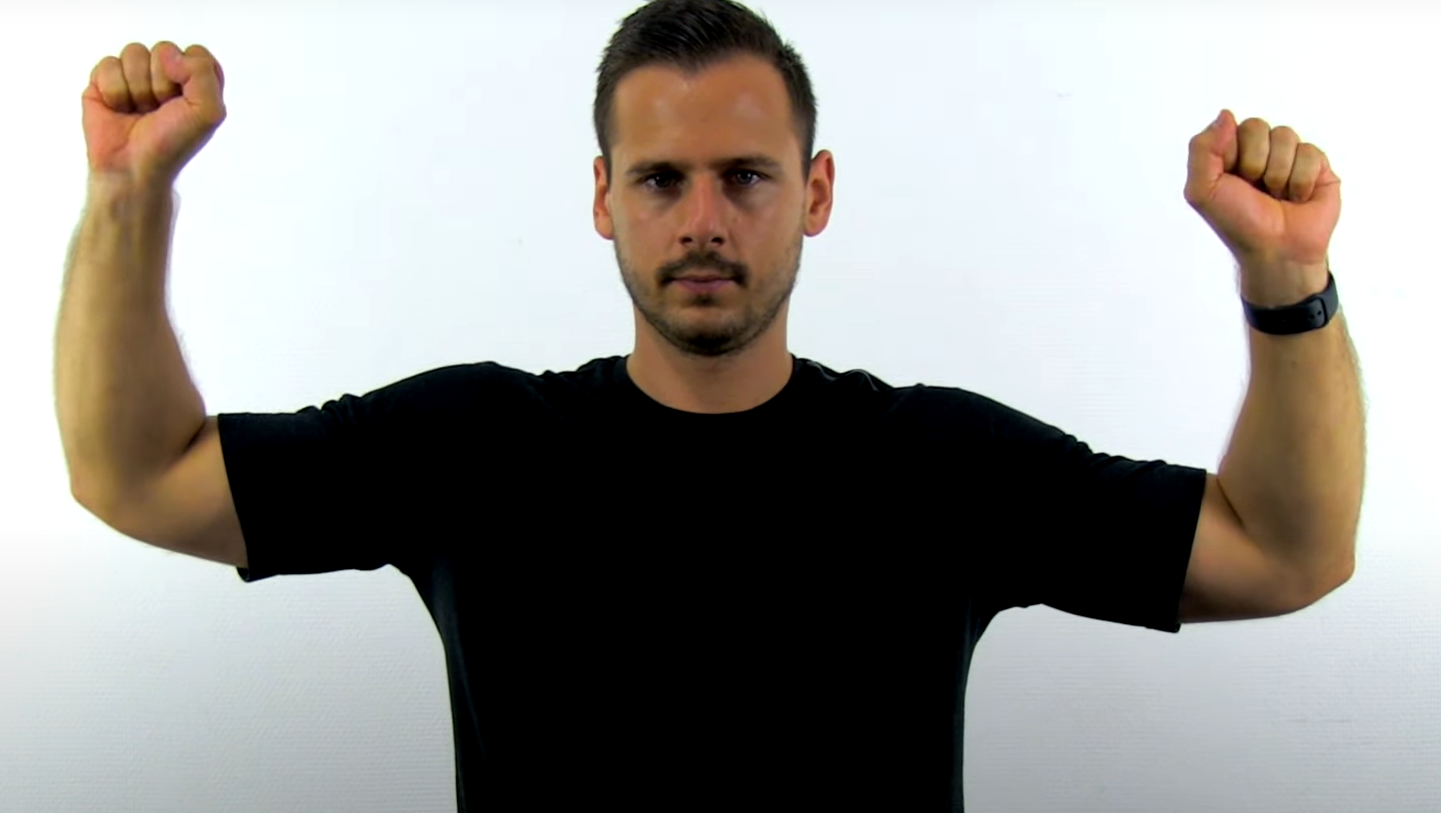
\includegraphics[keepaspectratio]{pad0.png}}

}

\caption{Roos Stress Test Position}

\end{figure}%

Ask the patient to \textbf{abduct his shoulders to 90 degrees}, with
\textbf{maximal external rotation} on.\\
Test is positive when patient \emph{can't keep this for more than 3
minutes}.

\begin{itemize}
\tightlist
\item[$\square$]
  \textbf{Allen's Test}\\
\item[$\square$]
  \textbf{Raynaud's}\\
\item[$\square$]
  \textbf{Ankle brachial pressure index}
\end{itemize}

\begin{tcolorbox}[enhanced jigsaw, left=2mm, toptitle=1mm, breakable, title=\textcolor{quarto-callout-note-color}{\faInfo}\hspace{0.5em}{Note}, coltitle=black, opacitybacktitle=0.6, arc=.35mm, colback=white, leftrule=.75mm, toprule=.15mm, bottomtitle=1mm, titlerule=0mm, rightrule=.15mm, colbacktitle=quarto-callout-note-color!10!white, bottomrule=.15mm, opacityback=0, colframe=quarto-callout-note-color-frame]

\textbf{Ankle Brachial Pressure Index (ABPI)}\\
It is a ratio between the blood pressure measured in the ankle and that
measured in the brachial artery, used to assess lower limb perfusion.

\begin{itemize}
\tightlist
\item
  Left ABPI = (Highest pressure of either left Post. tibial artery or
  left dorsalis pedis) / (Highest brachial pressure (R/L))\\
\item
  Right ABPI = (Highest pressure of either right Post. tibial artery or
  right dorsalis pedis) / (Highest brachial pressure (R/L))
\end{itemize}

\textbf{Normal ranges:}\\
- Normal → \(0.8 - 1.3\)\\
- Mild or moderate arterial disease → \(0.5 - 0.79\)
(\emph{claudication})\\
- Severe arterial disease → \(<0.5\) (\emph{Rest pain, ulceration,
gangrene → critical limb ischemia})\\
- Calcified vessels → \(>1.3\) (\emph{suggestive of DM, vasculitis,
atherosclerosis → need duplex US/CT angio})

\end{tcolorbox}

\bookmarksetup{startatroot}

\chapter{Cranial Nerve Examination
checklist}\label{cranial-nerve-examination-checklist}

\section{WIPPER and the Intro}\label{wipper-and-the-intro-7}

\begin{itemize}
\tightlist
\item[$\square$]
  Introduce yourself and shake hands
\item[$\square$]
  Washing of hands and appropriate hand hygiene
\item[$\square$]
  Asking for permission
\item[$\square$]
  Ensuring the room's privacy
\item[$\square$]
  Ensuring the environmental warmth and good lighting conditions
\item[$\square$]
  Asking for appropriate exposure (Head and neck)
\item[$\square$]
  Asking the patient to be in the appropriate position (Sitting on a
  chair)
\item[$\square$]
  Relocating to the right side of the patient
\item[$\square$]
  Asking for a chaperon
\item[$\square$]
  ``I have all of my equipment's''
\end{itemize}

\section{Olfactory Nerve Examination
(Useless)}\label{olfactory-nerve-examination-useless}

\begin{itemize}
\tightlist
\item[$\square$]
  Check the nasal passage
\item[$\square$]
  Ask the patient to close his eyes
\item[$\square$]
  Close one nostril to test the other
\item[$\square$]
  Ask the patient to smell (Use scratch and sniff test cards from UPSIT
  test)
\item[$\square$]
  Close the other nostril and repeat
\end{itemize}

\section{Optic Nerve Examination}\label{optic-nerve-examination}

\subsubsection{Inspection}\label{inspection-4}

\begin{itemize}
\tightlist
\item[$\square$]
  Comment on no head tilt
\item[$\square$]
  Comment on no facial asymmetry
\item[$\square$]
  Comment on no proptosis
\item[$\square$]
  Comment on no lid retraction
\item[$\square$]
  Do lid lag test, stand up and ask the patient to follow your finger,
  move it up and back, bottom and back, and comment on no lid lag
\end{itemize}

\subsubsection{Palpation}\label{palpation-5}

\begin{itemize}
\tightlist
\item[$\square$]
  Do the usuals for palpation
\item[$\square$]
  Comment on no tenderness over the eyes
\end{itemize}

\subsubsection{Tests to Mention}\label{tests-to-mention}

\begin{itemize}
\tightlist
\item[$\square$]
  ``I will assess visual acuity using Snellen's chart''
\item[$\square$]
  ``I will assess color vision using Isihara plates''
\item[$\square$]
  ``I will assess macular sparing using Amsler's grid''
\item[$\square$]
  ``I will do fundoscopy examination for things like optic disk
  examination, papilledema etc.''
\end{itemize}

\subsection{Pupillary Reflexes Tests}\label{pupillary-reflexes-tests}

\begin{itemize}
\tightlist
\item[$\square$]
  Dim the room and check the pupils' size for anisocorea
\item[$\square$]
  Ask the patient to fixate his eye on a distant point
\item[$\square$]
  Get your torch, slide it horizontally to one eye, notice ``Direct''
  reflex, then look at the other eye for ``Indirect/consensual'' reflex
\item[$\square$]
  Comment on intact direct and indirect pupillary reflexes
\item[$\square$]
  While patient is fixating, put your finger \textasciitilde15cm in
  front, ask him to focus on it and notice ``Convergence''
\item[$\square$]
  Comment on normal accommodation reflex
\end{itemize}

\subsection{Visual Field Tests}\label{visual-field-tests}

\begin{itemize}
\tightlist
\item[$\square$]
  Ask the patient to look at your eyes
\item[$\square$]
  Hold 1 hand at full extent, wiggle fingers and ask if patient sees
  movement
\item[$\square$]
  Test at 2, 4, 8 and 10 o'clock positions
\item[$\square$]
  Comment no homonymous visual field defect
\item[$\square$]
  For sensory inattention: hold both hands at 2 and 10 o'clock, wiggle
  one then both
\item[$\square$]
  Comment no sensory inattention
\end{itemize}

\subsection{Peripheral Visual Fields (one eye at a
time)}\label{peripheral-visual-fields-one-eye-at-a-time}

\begin{itemize}
\tightlist
\item[$\square$]
  Perform 1 eye closing maneuver
\item[$\square$]
  Ask patient to look at your eyes
\item[$\square$]
  Test each quadrant (2,4,8,10 o'clock) with finger wiggling
\item[$\square$]
  Test the other eye
\item[$\square$]
  Comment no peripheral visual field defects
\end{itemize}

\subsection{Color Desaturation}\label{color-desaturation}

\begin{itemize}
\tightlist
\item[$\square$]
  Show red object to ensure patient sees it red
\item[$\square$]
  Perform 1 eye closing maneuver
\item[$\square$]
  Place red object in front of open eye, ask about color
\item[$\square$]
  Test the other eye
\item[$\square$]
  Comment ``No red desaturation''
\end{itemize}

\subsection{Central Visual Field}\label{central-visual-field}

\begin{itemize}
\tightlist
\item[$\square$]
  Perform 1 eye closing maneuver
\item[$\square$]
  Ask patient to look at your eyes
\item[$\square$]
  Move red object from side to center until color is noticed
\item[$\square$]
  Test the other eye
\item[$\square$]
  Comment no central visual field defects
\end{itemize}

\subsection{Blind Spot}\label{blind-spot}

\begin{itemize}
\tightlist
\item[$\square$]
  Perform 1 eye closing maneuver
\item[$\square$]
  Ask patient to look at your eyes
\item[$\square$]
  Move red object horizontally until it disappears
\item[$\square$]
  Test the other eye
\item[$\square$]
  Comment on normal blind spot size
\end{itemize}

\section{Ocular Movement Nerves (3rd, 4th,
6th)}\label{ocular-movement-nerves-3rd-4th-6th}

\begin{itemize}
\tightlist
\item[$\square$]
  Ask patient to fix head and only move eyeballs following your finger
\item[$\square$]
  Draw H shape, observe eye movements
\item[$\square$]
  Ask about diplopia and its features if present
\item[$\square$]
  Comment on no nystagmus, no diplopia, full range of motion
\end{itemize}

\section{Trigeminal Nerve}\label{trigeminal-nerve}

\subsubsection{Sensory}\label{sensory}

\begin{itemize}
\tightlist
\item[$\square$]
  Test light touch on V1,V2,V3 areas bilaterally with cotton-wool
\item[$\square$]
  Repeat with neural tip for superficial pain
\item[$\square$]
  Mention testing general sensation on anterior 2/3 of tongue
\item[$\square$]
  Comment on intact symmetrical sensation
\end{itemize}

\subsubsection{Motor}\label{motor}

\begin{itemize}
\tightlist
\item[$\square$]
  Palpate/inspect temporalis for wasting
\item[$\square$]
  Ask patient to clench teeth, check masseters
\item[$\square$]
  Ask patient to open mouth, inspect for jaw deviation
\item[$\square$]
  Comment no muscle wasting, good bulk, no deviation
\end{itemize}

\subsubsection{Reflexes}\label{reflexes}

\begin{itemize}
\tightlist
\item[$\square$]
  For jaw reflex: place finger between lower lip/chin, percuss with
  hammer
\item[$\square$]
  Comment on normal jaw reflex
\item[$\square$]
  Mention testing corneal reflex
\end{itemize}

\section{Facial Nerve}\label{facial-nerve}

\subsubsection{Motor}\label{motor-1}

\begin{itemize}
\tightlist
\item[$\square$]
  Ask patient to raise eyebrows, assess symmetry (frontalis)
\item[$\square$]
  Comment symmetrical wrinkles
\item[$\square$]
  Ask patient to forcefully close eyes against resistance
\item[$\square$]
  Comment normal power of orbicularis oculi
\item[$\square$]
  Ask patient to ``Blow out your cheeks and don't let me deflate them''
\item[$\square$]
  Comment normal power of buccinator/orbicularis oris
\item[$\square$]
  Ask patient to show teeth (smile)
\item[$\square$]
  Comment symmetry and no mouth angle deviation
\end{itemize}

\subsubsection{Sensory}\label{sensory-1}

\begin{itemize}
\tightlist
\item[$\square$]
  Test touch sensation behind ear
\item[$\square$]
  Mention testing taste on anterior 2/3 of tongue
\item[$\square$]
  Mention corneal reflex
\item[$\square$]
  Ask about hearing changes (stapedius muscle)
\end{itemize}

\section{Vestibulocochlear Nerve}\label{vestibulocochlear-nerve}

\subsubsection{Hearing Tests}\label{hearing-tests}

\begin{itemize}
\tightlist
\item[$\square$]
  Stand behind patient, ensure normal hearing first
\item[$\square$]
  Close one ear, whisper at 60cm, ask patient to repeat
\item[$\square$]
  If needed, whisper at 15cm
\end{itemize}

\subsubsection{Weber's Test}\label{webers-test}

\begin{itemize}
\tightlist
\item[$\square$]
  Tap 512Hz fork, place on forehead midline
\item[$\square$]
  Ask if sound is louder in any ear
\item[$\square$]
  Comment negative Weber's test (no lateralization)
\end{itemize}

\subsubsection{Rinne's Test}\label{rinnes-test}

\begin{itemize}
\tightlist
\item[$\square$]
  Tap 512Hz fork, place on mastoid prominence
\item[$\square$]
  Ask patient to signal when sound stops
\item[$\square$]
  Move fork near ear, ask if sound returns
\item[$\square$]
  Comment positive Rinne's test (air\textgreater bone conduction)
\end{itemize}

\section{Glossopharyngeal and Vagus
Nerves}\label{glossopharyngeal-and-vagus-nerves}

\begin{itemize}
\tightlist
\item[$\square$]
  Ask patient to talk, note no dysphonia/dysarthria
\item[$\square$]
  Ask patient to say ``aah'', check uvula
\item[$\square$]
  Comment no uvula deviation
\item[$\square$]
  Ask patient to puff cheeks, listen for nasal regurgitation
\item[$\square$]
  Comment no nasal regurgitation
\item[$\square$]
  Ask patient to cough (assess for bovine cough)
\item[$\square$]
  Mention testing gag reflex
\item[$\square$]
  Mention giving water to assess swallowing
\item[$\square$]
  Mention testing taste on posterior 1/3 of tongue
\end{itemize}

\section{Accessory Nerve}\label{accessory-nerve}

\begin{itemize}
\tightlist
\item[$\square$]
  Inspect SCM and trapezius
\item[$\square$]
  Comment no wasting/asymmetry in trapezius
\item[$\square$]
  Palpate both muscles for bulk
\item[$\square$]
  Comment normal bulk
\item[$\square$]
  Test trapezius power: shrug shoulders against resistance
\item[$\square$]
  Comment normal trapezius power
\item[$\square$]
  Test SCM power: turn head against resistance
\item[$\square$]
  Test other SCM
\item[$\square$]
  Test bilateral SCM: look down against chin resistance
\item[$\square$]
  Comment normal SCM power
\end{itemize}

\section{Hypoglossal Nerve}\label{hypoglossal-nerve}

\begin{itemize}
\tightlist
\item[$\square$]
  Ask patient to open mouth, inspect tongue
\item[$\square$]
  Comment no wasting/fasciculations
\item[$\square$]
  Ask patient to protrude tongue, check deviation
\item[$\square$]
  Comment no deviation/fasciculations
\item[$\square$]
  Ask patient to move tongue side-to-side quickly
\item[$\square$]
  Comment normal movement
\item[$\square$]
  Ask patient to press tongue against cheek, assess power
\item[$\square$]
  Comment normal power
\item[$\square$]
  Assess speech with ``Yellow lorry'' etc.
\item[$\square$]
  Comment normal speech
\item[$\square$]
  Mention testing swallowing
\end{itemize}

THE END

\bookmarksetup{startatroot}

\chapter{Miscellaneous}\label{miscellaneous}

\subsection{\texorpdfstring{\emph{The 3 questions in \textbf{general
look of the
patient}}}{The 3 questions in general look of the patient}}\label{the-3-questions-in-general-look-of-the-patient}

\begin{enumerate}
\def\labelenumi{\arabic{enumi}.}
\item
  Do you know who I am?
\item
  Do you know where you are?
\item
  Do you know what time it is?
\end{enumerate}

\subsection{\texorpdfstring{\emph{The 6 vital
signs}}{The 6 vital signs}}\label{the-6-vital-signs}

\begin{enumerate}
\def\labelenumi{\arabic{enumi}.}
\tightlist
\item
  \emph{Heart rate (pulse rate)} (\(60 - 100\) beat per minute)
\item
  \emph{Blood pressure}
\item
  \emph{Respiratory rate} (\(12-20\) breath per minute)
\item
  \emph{Oxygen concentration} (SpO₂) (\(\geq 95\%\) or 88\%-92\% if
  COPD)
\item
  \emph{Body temperature} (*\(36.5\leq x \leq37.2\))
\item
  \emph{Pain score out of \(10\)}
\end{enumerate}

\subsection{\texorpdfstring{\emph{The usuals for
palpation}}{The usuals for palpation}}\label{the-usuals-for-palpation}

\begin{enumerate}
\def\labelenumi{\arabic{enumi}.}
\tightlist
\item
  Mention that your hands are warm and clean (you can also rub your
  hands together to warm them, re-apply hygiene too)
\item
  Ask about pain in the area you're about to palpate, hold eye contact
  and begin
\end{enumerate}

\subsection{\texorpdfstring{\emph{The 5F's of abdominal
distension}}{The 5F's of abdominal distension}}\label{the-5fs-of-abdominal-distension}

\begin{enumerate}
\def\labelenumi{\arabic{enumi}.}
\tightlist
\item
  Fetus \emph{(Pregnancy)}
\item
  Flatus \emph{(Any cause of bloating such as IBS..etc)}
\item
  Feces \emph{(Constipation)}
\item
  Fluid \emph{(Any cause such as ascites of chronic liver disease)}
\item
  Fat
\end{enumerate}




\end{document}
